\documentclass[10pt,journal,compsoc]{IEEEtran}

\usepackage{amsmath,amssymb,amsfonts}
\usepackage{algorithmic}
\usepackage{graphicx}
\usepackage{textcomp}
\usepackage{xcolor}
\usepackage{booktabs}
\usepackage{multirow}
\usepackage{url}
\usepackage{hyperref}
\usepackage{microtype}

\hypersetup{
    colorlinks=true,
    linkcolor=blue,
    citecolor=blue,
    urlcolor=blue
}

\begin{document}

\title{Foundation Models and Reasoning LLMs for Scientific Multimodal Time Series: A Survey}

\author{Huirui~Li%
\thanks{H. Li is with the School of Data Science and Artificial Intelligence. Correspondence e-mail: 58367737+lihuirui@users.noreply.github.com.}%
\thanks{Manuscript version 1.0 (P0/P1 Bootstrap Iteration), September 24, 2026.}
}

\IEEEtitleabstractindextext{%
\begin{abstract}
Time series and spatio-temporal dynamics arising in natural systems---such as global weather, long-term climate, hydrological flood regimes, ocean circulation, earthquake wave propagation, satellite earth observations, and heliophysical radiation---differ fundamentally from generic tabular or urban traffic series. They are governed by continuous non-linear partial differential equations, multi-scale turbulent interactions, heterogeneous spatial geometries, and strict physical conservation laws. Recently, the emergence of pre-trained foundation models (PFMs) and scientific reasoning Large Language Models (LLMs) has instigated a paradigm shift across computational earth and physical sciences. This survey provides the first comprehensive, systematic review of foundation models and reasoning LLMs tailored for scientific multimodal time series. Guided by the PRISMA 2020 methodology, we review landmark architectures developed between 2021 and 2026 across major natural science domains. We introduce a systematic taxonomy structured along four orthogonal axes: (1) scientific domains and multimodal data representations, (2) foundation model architectural backbones (including 3D spherical transformers, multi-mesh graph neural networks, continuous neural operators, and generative diffusion ensembles), (3) levels of physical law integration (from purely data-driven to soft physical penalties and hybrid PDE solvers), and (4) functional roles of LLMs in scientific reasoning (as direct predictors, contextual enhancers, and autonomous tool-orchestrating agents). Furthermore, we curate standardized operational evaluation protocols (such as WeatherBench 2 and SciTS), contrast model scale against forecast horizon, and identify crucial open frontiers spanning universal cross-physics tokenization, physical conservation guarantees, and trustworthy autonomous scientific discovery.
\end{abstract}

\begin{IEEEkeywords}
Scientific Foundation Models, Multimodal Time Series, Spatio-Temporal Modeling, Large Language Models, Scientific Reasoning, Weather and Climate Forecasting, Physics-Informed Machine Learning.
\end{IEEEkeywords}}

\maketitle
\IEEEdisplaynontitleabstractindextext
\IEEEpeerreviewmaketitle

\section{Introduction}
\label{sec:introduction}

Temporal and spatio-temporal dynamics constitute the empirical foundation of the natural sciences. From the planetary atmospheric circulation driving global weather patterns to the sub-surface acoustic vibrations heralding seismic rupture, physical processes unfold across continuous temporal trajectories and multi-scale spatial coordinates. Over the past several decades, the modeling and prediction of these scientific phenomena have predominantly relied on Numerical Weather Prediction (NWP) and classical numerical differential equation solvers, such as the Integrated Forecasting System (IFS) maintained by the European Centre for Medium-Range Weather Forecasts (ECMWF) and finite-difference hydrodynamic models. While physically principled, numerical solvers incur colossal computational burdens, requiring massive supercomputing clusters to perform high-resolution discretization and step-by-step numerical integration.

In parallel, the broader machine learning community has witnessed a revolution driven by pre-trained foundation models (PFMs) and Large Language Models (LLMs). While foundational models initially transformed natural language processing and computer vision, their underlying principles---self-supervised pretraining on planetary-scale corpora, emergent scaling behaviors, and zero-shot downstream transferability---have rapidly migrated into temporal data mining. Earlier general surveys, notably the seminal work by Jin et al.~\cite{jin2023largemodels} and its position sequel~\cite{jin2024whatcan}, comprehensively charted large models for general time series analysis (LM4TS) and spatio-temporal data mining (LM4STD). However, as highlighted in Table~\ref{tab:survey_comparison}, existing overviews focus heavily on urban computing, human mobility trajectories, traffic sensor networks, and generic 1D benchmark datasets (e.g., electricity, weather station benchmarks, exchange rates).

\begin{table*}[t]
\centering
\caption{Comparison of This Survey with Existing Literature and Related Temporal Surveys.}
\label{tab:survey_comparison}
\scriptsize
\setlength{\tabcolsep}{4pt}
\begin{tabular}{@{}lp{0.6cm}p{2.2cm}p{2.0cm}p{3.2cm}p{2.0cm}p{3.6cm}@{}}
\toprule
\textbf{Survey / Study} & \textbf{Year} & \textbf{Scope Focus} & \textbf{Physical Grounding} & \textbf{Multimodal Modalities} & \textbf{LLM Reasoning} & \textbf{Core Domains Covered} \\
\midrule
Jin et al.~\cite{jin2023largemodels} & 2023 & General Spatio-Temporal & Moderate & General Multimodal & Limited & Urban traffic, human trajectory, generic time series \\
Jin et al.~\cite{jin2024whatcan} & 2024 & LLM for Time Series & Low & Text + 1D Series & Moderate (Position) & Benchmark time series forecasting, tokenization \\
Rasp et al.~\cite{rasp2024weatherbench2} & 2024 & Weather Benchmark & High (Meteorology) & Gridded NWP Reanalysis & None & Global numerical and ML weather forecasting \\
\textbf{This Survey} & \textbf{2026} & \textbf{Scientific Multimodal} & \textbf{High (PDEs \& Laws)} & \textbf{Gridded + Satellite + Waveforms + Text} & \textbf{Comprehensive (Agents \& SciTS)} & \textbf{Weather/Climate, Earth Observation, Hydrology, Oceans, Seismology, Heliophysics} \\
\bottomrule
\end{tabular}
\end{table*}

Natural physical systems diverge fundamentally from human-generated temporal sequences across several intrinsic dimensions:
\begin{enumerate}
    \item \textbf{Governing Physical Laws and Conservation Constraints}: Physical time series are bounded by fundamental conservation laws of mass, energy, momentum, and moisture flux. Models that learn purely statistical correlations often generate unphysical states, such as negative precipitation or violation of energy conservation over extended rollouts.
    \item \textbf{High-Dimensional Multimodal Representations}: Scientific investigations integrate heterogeneous observation modalities, including 3D atmospheric pressure tensors (e.g., ERA5 reanalysis with geopotential height, temperature, and wind fields), multi-spectral satellite imagery (e.g., Sentinel-2, Landsat), river gauge discharge records, and continuous seismic waveforms.
    \item \textbf{Continuous Spatio-Temporal Geometries}: The Earth is a non-Euclidean spherical geometry with topological singularities at the poles, rendering standard 2D Euclidean convolutions and planar patch projections geometrically distorted.
    \item \textbf{The Need for Scientific Reasoning and Autonomous Discovery}: Beyond numerical point prediction, domain scientists demand causal attribution, physical hypothesis testing, and interactive tool orchestration. This has catalyzed the emergence of scientific reasoning LLMs and autonomous scientific agents capable of operating over complex temporal data.
\end{enumerate}

To bridge this literature gap, this survey delivers the first systematic, domain-science-centered investigation of foundation models and reasoning LLMs developed for scientific multimodal time series. We synthesize breakthroughs from 2021 through 2026 across atmospheric sciences, Earth observation, hydrology, oceanography, seismology, and heliophysics.

\subsection{Contributions of This Survey}
The primary contributions of this survey are summarized as follows:
\begin{itemize}
    \item \textbf{Domain-Science Centered Scoping}: We delimit the survey strictly to natural physical systems, explicitly analyzing the coupling between continuous physics, governing equations, and deep representation architectures.
    \item \textbf{Four-Dimensional Taxonomy Framework}: We establish an orthogonal classification scheme covering (1) Scientific Domains and Modalities, (2) Foundation Model Architectures, (3) Physics Integration Levels, and (4) Functional Roles of Reasoning LLMs.
    \item \textbf{Systematic Review Protocol}: Adhering to PRISMA 2020 standards, every candidate study is screened against strict empirical criteria and validated via official academic API records.
    \item \textbf{Synthesis of Evaluation Protocols and Frontiers}: We analyze standardized scientific benchmarks (such as WeatherBench 2 and SciTS), map spatial resolution against maximum forecast lead time, and delineate critical open challenges in physical conservation, multi-physics tokenization, and autonomous scientific discovery.
\end{itemize}

\section{Background and Preliminaries}
\label{sec:background}

\subsection{Formal Data Modality Formulations}
Scientific multimodal temporal datasets exhibit diverse mathematical structures depending on observation platforms, sensing geometries, and sampling frequencies. We formalize the four dominant scientific temporal modalities as follows:

\subsubsection{In-Situ Station and Gauge Time Series}
Discrete ground monitoring networks (e.g., weather stations, hydrological streamflow gauges, ocean buoys) record continuous physical variables at fixed geospatial coordinates $(u_i, v_i)$. An in-situ observation sequence is defined as:
\begin{equation}
    \mathbf{X}^{(i)} = \{ \mathbf{x}_t^{(i)} \in \mathbb{R}^{C_{\text{station}}} \}_{t=1}^{T},
\end{equation}
where $T$ represents the temporal horizon and $C_{\text{station}}$ denotes the recorded physical channels (e.g., precipitation, river discharge, 2-meter air temperature).

\subsubsection{Gridded Global/Regional Reanalysis Tensors}
Atmospheric and oceanic numerical simulations discretize the planetary sphere $\mathbb{S}^2$ into a regular latitude-longitude grid with $H$ latitudinal points and $W$ longitudinal points across $L$ vertical vertical pressure levels. The state tensor at time step $t$ is expressed as:
\begin{equation}
    \mathcal{X}_t \in \mathbb{R}^{H \times W \times L \times C_{\text{grid}}},
\end{equation}
where $C_{\text{grid}}$ incorporates upper-air variables (geopotential height $z$, temperature $T$, zonal and meridional wind components $u, v$, specific humidity $q$) alongside surface diagnostic fields (mean sea-level pressure $msl$, surface solar radiation).

\subsubsection{Multi-Spectral Remote Sensing Cubes}
Earth observation satellites (e.g., Sentinel-2, Landsat-8) capture surface reflectance over space, time, and electromagnetic spectral bands. A multi-temporal remote sensing observation cube is represented as:
\begin{equation}
    \mathcal{S}_{1:T} \in \mathbb{R}^{T \times B \times H_s \times W_s},
\end{equation}
where $B$ denotes the number of spectral bands (visible RGB, near-infrared, short-wave infrared, synthetic aperture radar polarization), and $(H_s, W_s)$ denotes the spatial pixel footprint.

\subsubsection{High-Frequency Continuous Waveforms}
Geophysical and seismological networks deploy seismometers recording ground motion acceleration or velocity across three orthogonal physical axes (Vertical $Z$, North-South $N$, East-West $E$). A continuous seismic waveform segment is formalized as:
\begin{equation}
    \mathbf{W} \in \mathbb{R}^{3 \times N_s},
\end{equation}
where $N_s = f_s \cdot \Delta \tau$ is the number of discrete digital samples collected at sampling frequency $f_s$ (typically 50--100 Hz).

\subsection{Core Problem Formulations}

\subsubsection{Deterministic Autoregressive Rollout Forecasting}
\begin{equation}
    \hat{\mathcal{X}}_{t+1:t+K} = \mathcal{M}_\theta(\mathcal{X}_{t-M+1:t}),
\end{equation}
optimized via latitude-weighted multi-step rollout loss:
\begin{equation}
    \mathcal{L}_{\text{det}} = \sum_{k=1}^K \lambda_k \|\hat{\mathcal{X}}_{t+k} - \mathcal{X}_{t+k}\|_{\mathbf{W}_{\text{lat}}}^2,
\end{equation}
where $\|\cdot\|_{\mathbf{W}_{\text{lat}}}$ represents a latitude-weighted norm accounting for spherical grid cell area convergence toward the poles:
\begin{equation}
    w_{\text{lat}}(i) = \frac{\cos(\phi_i)}{\frac{1}{H} \sum_{j=1}^H \cos(\phi_j)}.
\end{equation}

\subsubsection{Probabilistic Ensemble Generation}
Because chaotic atmospheric and oceanic dynamics exhibit sensitivity to initial conditions (the butterfly effect), deterministic point forecasts blur at longer lead times. Probabilistic foundation models aim to sample from the conditional predictive distribution:
\begin{equation}
    p_\theta(\mathcal{X}_{t+1:t+K} \mid \mathcal{X}_{t-M+1:t}),
\end{equation}
minimized using Continuous Ranked Probability Score (CRPS) or diffusion score-matching loss objectives~\cite{price2023gencast}.

\subsubsection{Scientific Question-Answering and Autonomous Reasoning}
Let $\mathcal{Q}$ represent a natural language scientific inquiry, and $\mathcal{D}_{\text{time}}$ represent an associated temporal or spatio-temporal data sequence. A scientific reasoning LLM $\mathcal{F}_{\text{LLM}}$ generates explanatory reasoning chains and structured conclusions $\mathcal{Y}$:
\begin{equation}
    \mathcal{Y} = \mathcal{F}_{\text{LLM}}(\mathcal{Q}, \mathcal{E}(\mathcal{D}_{\text{time}})),
\end{equation}
where $\mathcal{E}$ is a modality-specific continuous tokenizer or latent temporal encoder~\cite{wu2025scits}.

\section{Taxonomy and Overview}
\label{sec:taxonomy}

To systematically classify the rapidly expanding body of literature on scientific multimodal time series foundation models and reasoning LLMs, we construct a four-dimensional taxonomy framework, as illustrated in Fig.~\ref{fig:taxonomy_tree}. Unlike general-purpose temporal surveys that divide models simply by task (e.g., forecasting vs. imputation), our categorization captures the unique physical, mathematical, and algorithmic requirements of scientific domain applications.

\begin{figure*}[t]
\centering
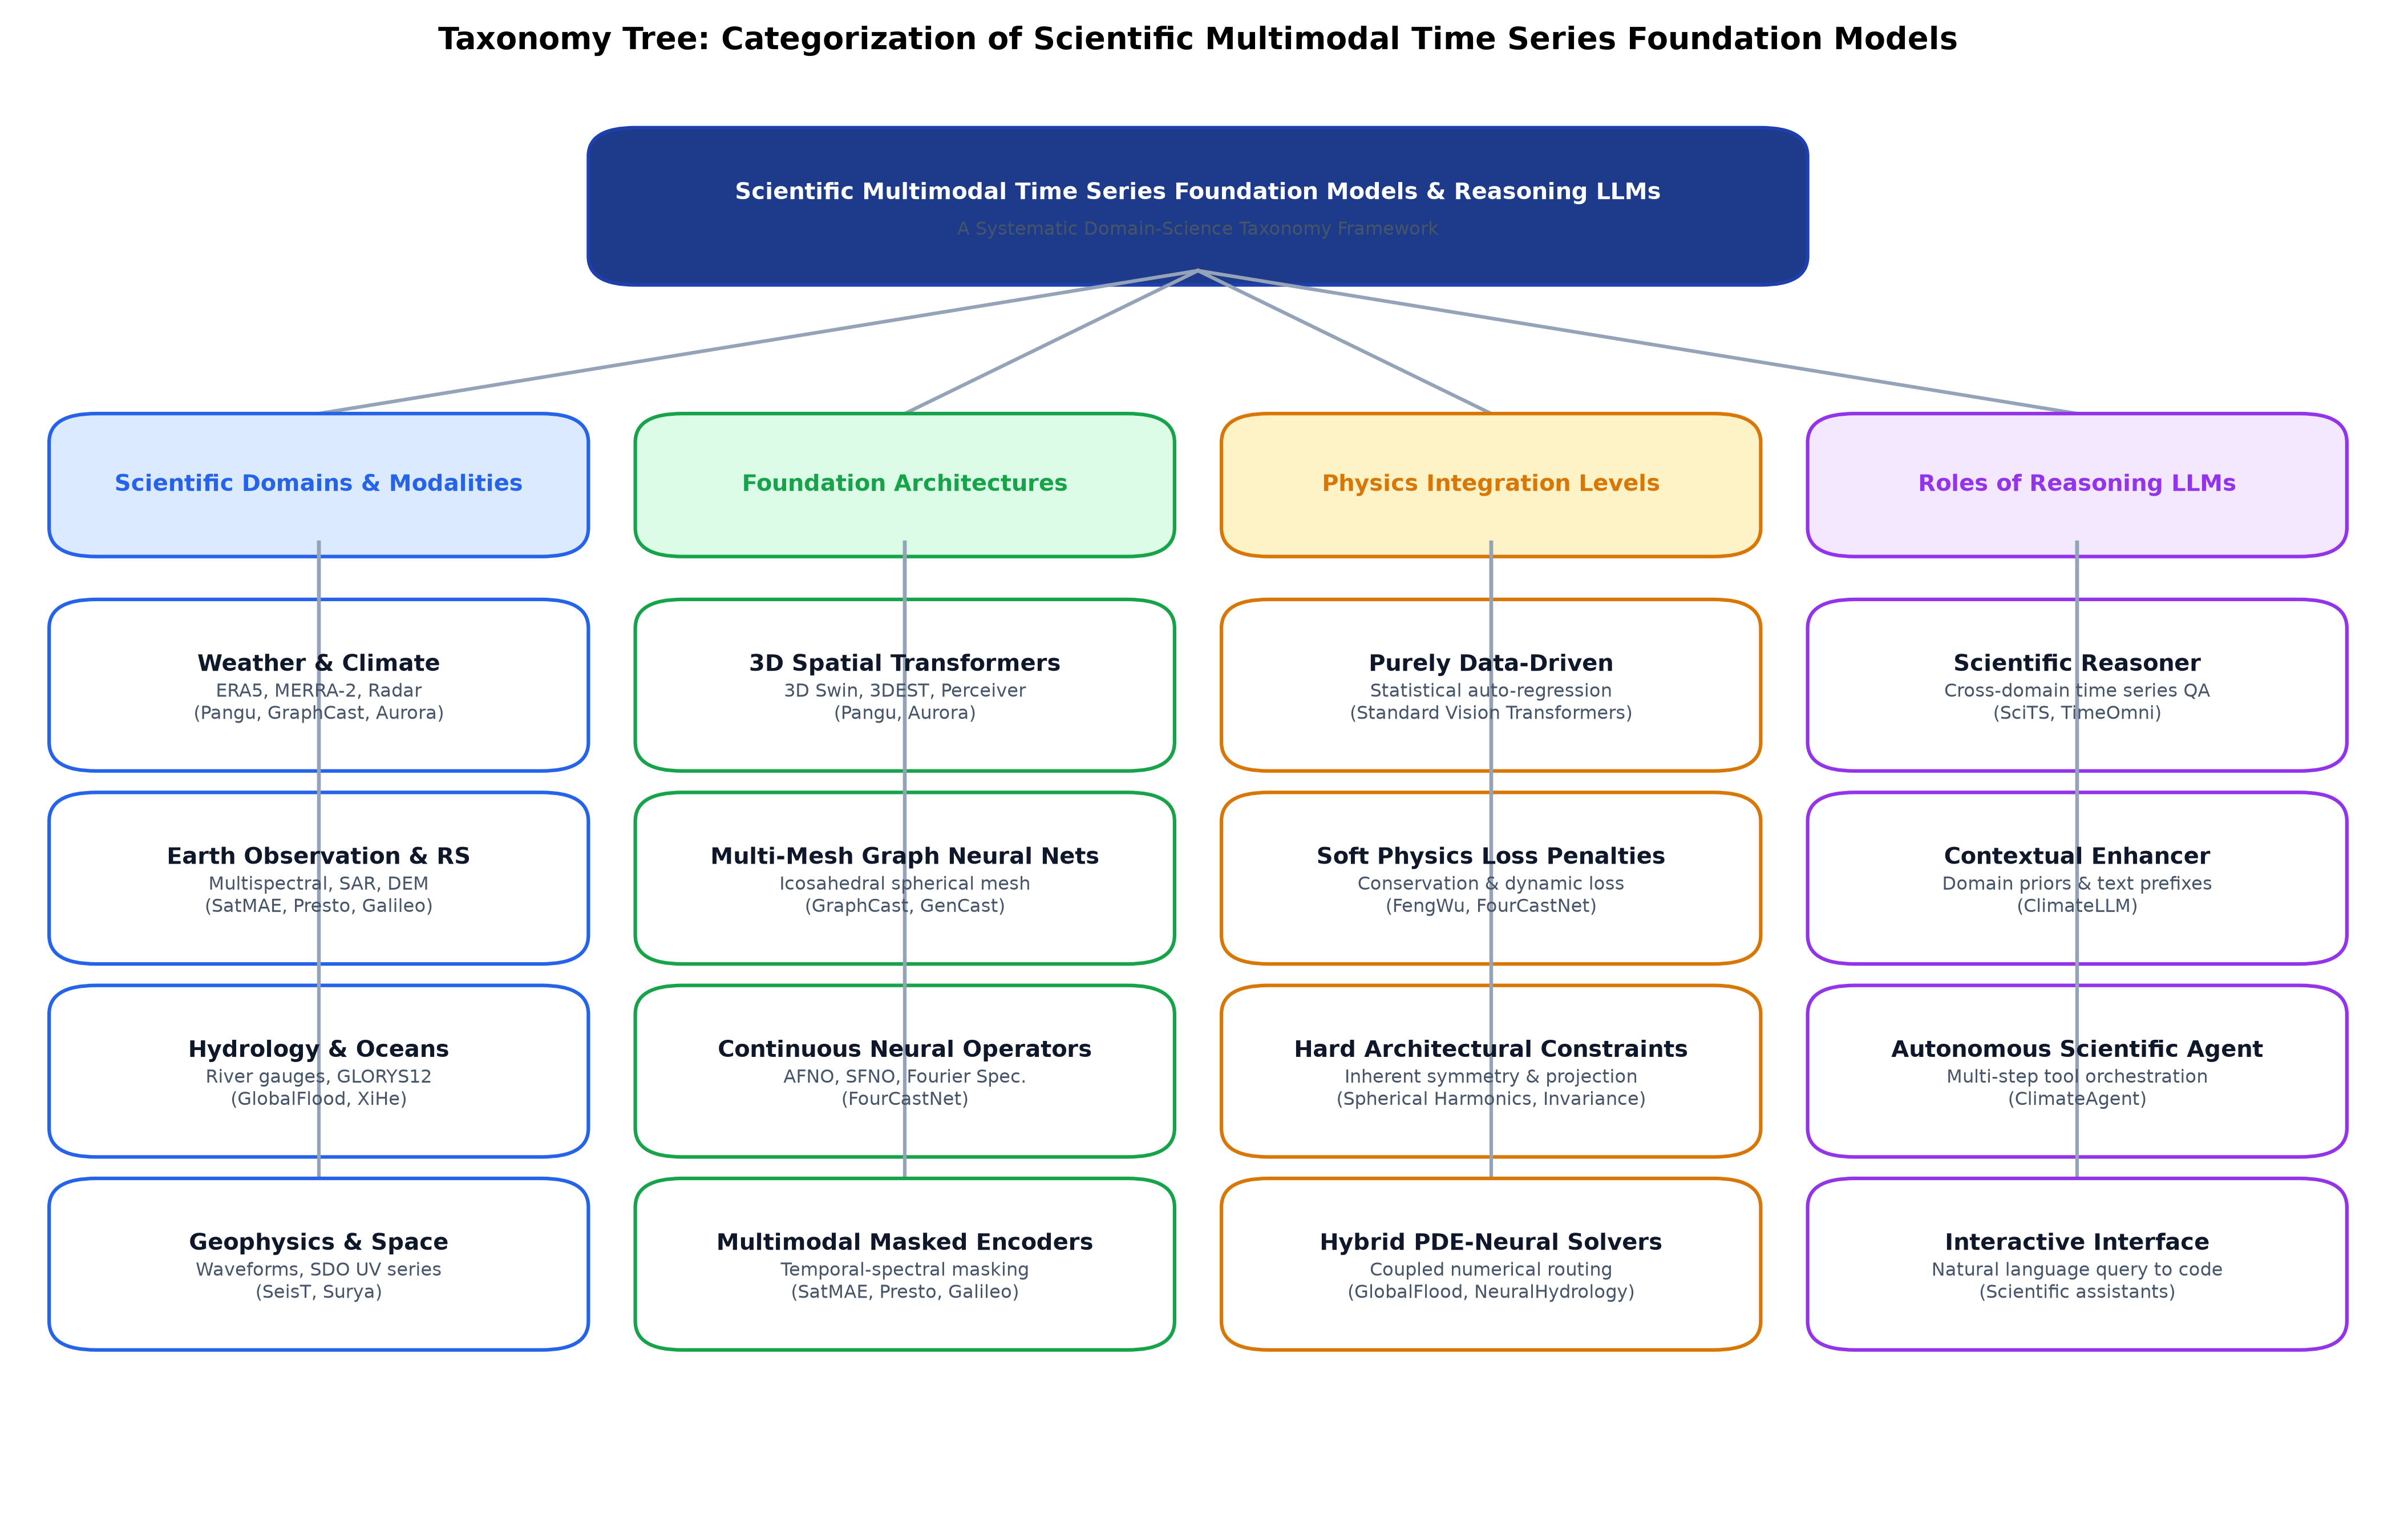
\includegraphics[width=\textwidth]{figures/taxonomy_tree.png}
\caption{Comprehensive taxonomy framework for scientific multimodal time series foundation models and reasoning LLMs, structured across four orthogonal dimensions: Scientific Domains \& Modalities, Foundation Architectures, Physics Integration Levels, and Roles of Reasoning LLMs.}
\label{fig:taxonomy_tree}
\end{figure*}

\subsection{Dimension 1: Scientific Domains and Modalities}
Scientific time series foundation models specialize across distinct physical environments:
\begin{itemize}
    \item \textbf{Weather and Climate}: Characterized by 3D spherical atmospheric reanalysis fields (ERA5, MERRA-2, IFS HRES), satellite radiometer scans, and ground radar nowcasting sequences~\cite{bi2023pangu,lam2023graphcast,pathak2022fourcastnet,bodnar2024aurora}.
    \item \textbf{Earth Observation and Remote Sensing}: Composed of irregular multi-spectral satellite revisit series (Sentinel-1 SAR, Sentinel-2 Optical, Landsat-8), high-resolution elevation maps, and surface reflectance temporal trajectories~\cite{cong2022satmae,tseng2023presto,tseng2025galileo,jakubik2023prithvi,brown2025alphaearth}.
    \item \textbf{Hydrology and Water Resources}: Integrating multi-basin river streamflow gauges, topological river drainage networks, and gridded surface precipitation/evapotranspiration dynamics~\cite{nearing2024globalflood}.
    \item \textbf{Oceanography and Marine Systems}: Involving global eddy-resolving reanalysis fields (e.g., GLORYS12V1), sea surface height anomalies, temperature/salinity profiles, and acoustic sensor logs~\cite{wang2024xihe}.
    \item \textbf{Geophysics and Seismology}: Continuous 3-component seismic waveforms, phase arrival triggers, fault slip observations, and GPS tectonic deformation velocities~\cite{li2024seist,zhu2019phasenet}.
    \item \textbf{Space Weather and Heliophysics}: Continuous solar extreme ultraviolet (EUV) magnetograms, solar wind ion velocities, and geomagnetic disturbance indices~\cite{roy2025surya}.
\end{itemize}

As visualized in the Domain $\times$ Modality Research Maturity Matrix (Fig.~\ref{fig:domain_modality_heatmap}), while gridded weather reanalysis and multi-spectral satellite imagery have achieved high maturity, cross-modal integration (e.g., coupling continuous waveforms with satellite imagery or ground gauges with scientific text logs) remains an active frontier.

\begin{figure}[t]
\centering
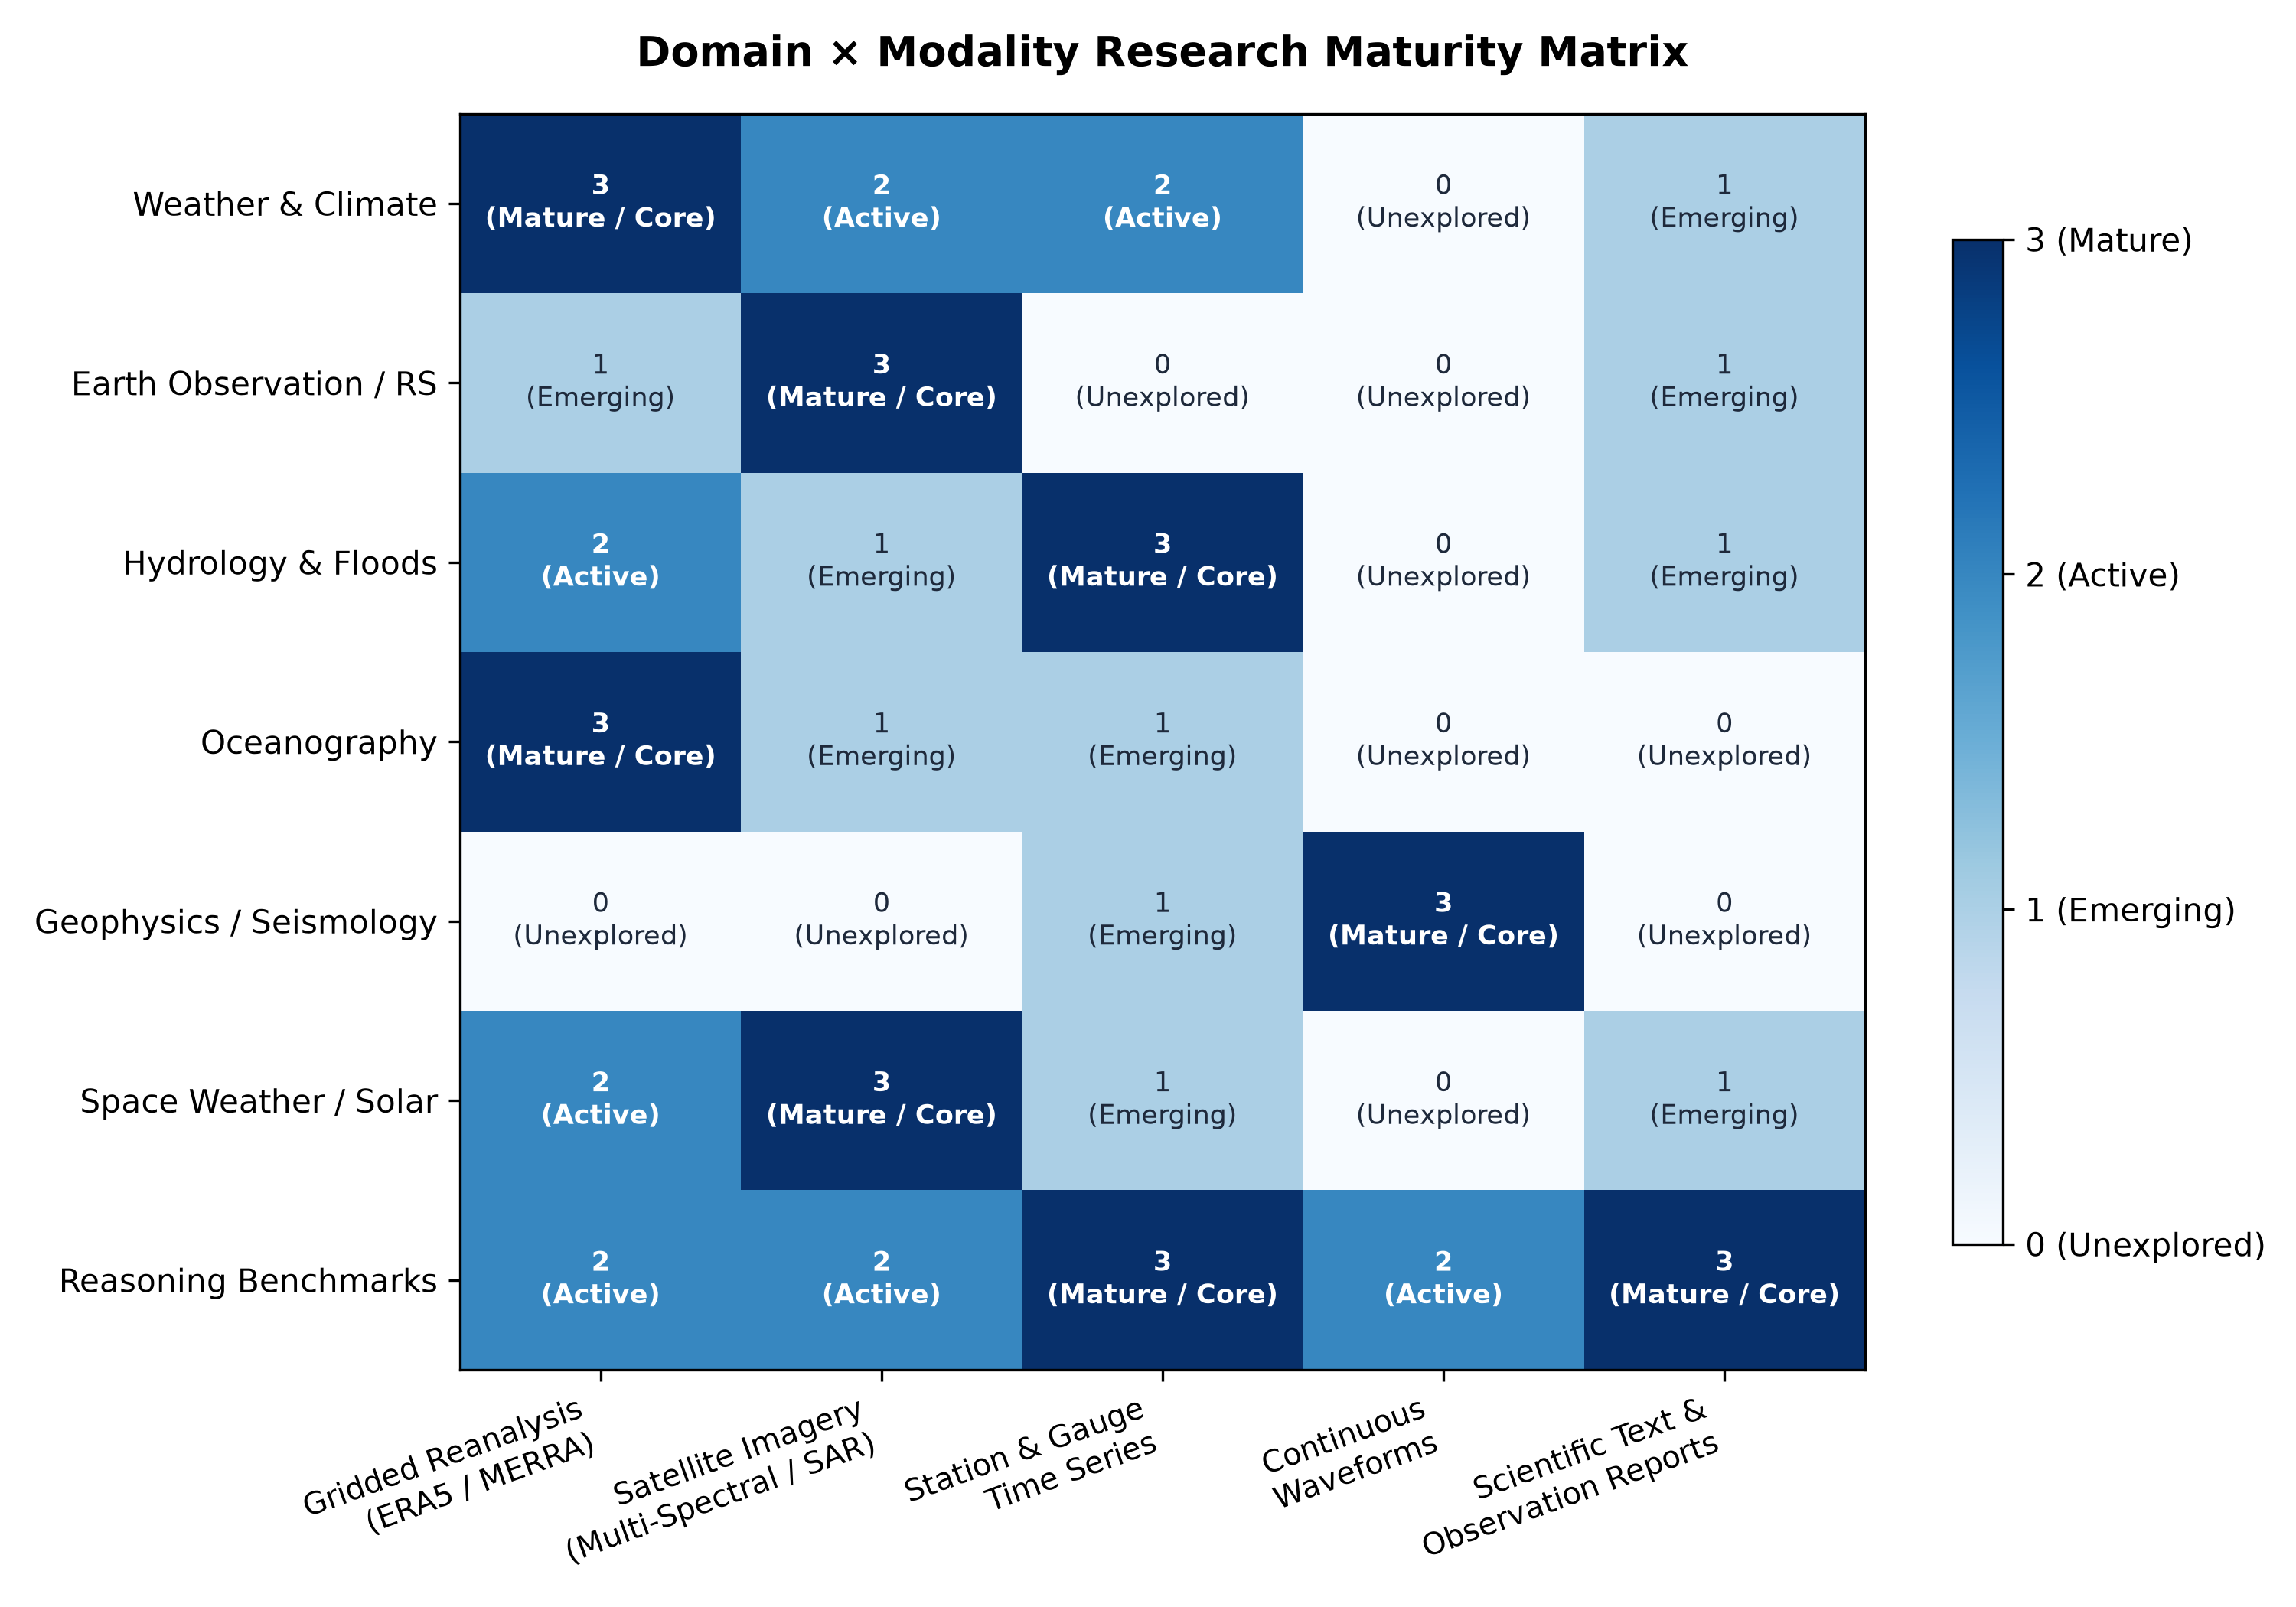
\includegraphics[width=\columnwidth]{figures/domain_modality_heatmap.png}
\caption{Domain $\times$ Modality Research Maturity Matrix, highlighting established core areas and emerging multimodal frontiers.}
\label{fig:domain_modality_heatmap}
\end{figure}

\subsection{Dimension 2: Foundation Model Architectures}
We categorize foundation backbones by their spatial-temporal inductive biases:
\begin{itemize}
    \item \textbf{3D Spatial Transformers}: Employing 3D Earth-specific patch embeddings, hierarchical Swin-like windowed attention, and vertical pressure-level encodings~\cite{bi2023pangu,bodnar2024aurora,chen2023fuxi}.
    \item \textbf{Multi-Mesh Graph Neural Networks}: Discretizing the spherical Earth via refined recursive icosahedral meshes to ensure uniform spatial resolution without polar distortions~\cite{lam2023graphcast}.
    \item \textbf{Continuous Neural Operators}: Leveraging Fourier transforms and spectral convolutions (e.g., AFNO, SFNO) to learn discretization-invariant operators on function spaces~\cite{pathak2022fourcastnet}.
    \item \textbf{Multimodal Masked Autoencoders}: Extending masked autoencoding (MAE) across spatial patches, temporal revisit cycles, and spectral channel wavelengths~\cite{cong2022satmae,tseng2023presto,tseng2025galileo,jakubik2023prithvi}.
    \item \textbf{Generative Diffusion Models}: Utilizing score-based diffusion denoising to generate calibrated, physically perturbed probabilistic weather and extreme event ensembles~\cite{price2023gencast}.
\end{itemize}

\subsection{Dimension 3: Physics Integration Levels}
The physical fidelity of deep learning models ranges along four distinct levels:
\begin{enumerate}
    \item \textbf{Purely Data-Driven}: Models optimize statistical reconstruction (e.g., mean squared error, MAE) over historical datasets without explicit differential constraints, relying solely on model capacity to reflect physical dynamics.
    \item \textbf{Soft Physics Loss Penalties}: Physical conservation principles (e.g., kinetic energy conservation, mass balance, divergence-free constraints) are formulated as penalty terms within the training loss function~\cite{chen2023fengwu,pathak2022fourcastnet}.
    \item \textbf{Hard Architectural Conservation Constraints}: Structural projections (e.g., spherical harmonics basis expansion, divergence-free projection layers) guarantee that model predictions strictly satisfy conservation laws by construction.
    \item \textbf{Hybrid PDE-Neural Ensembles}: Deep neural representations predict intermediate flux states or residual tendencies coupled directly to numerical differential equation solvers~\cite{nearing2024globalflood}.
\end{enumerate}

\subsection{Dimension 4: Functional Roles of Reasoning LLMs}
Large Language Models engage with scientific temporal data through four operational archetypes:
\begin{itemize}
    \item \textbf{Scientific Reasoner}: Understanding physical time series tokens and generating natural language explanations, causal attribution, and hypothesis evaluation across scientific domains~\cite{wu2025scits}.
    \item \textbf{Contextual Enhancer}: Supplying auxiliary domain semantics, station metadata, and climate zone priors to guide numerical prediction backbones~\cite{li2025climatellm}.
    \item \textbf{Autonomous Tool-Using Agent}: Decomposing complex scientific inquiries, retrieving real-time sensor streams, and executing scientific diagnostic libraries (e.g., CDO, xarray, SciPy) to produce verified scientific analyses~\cite{li2025climateagent}.
    \item \textbf{Interactive Natural Language Interface}: Translating unstructured scientist inquiries into executable database queries and simulation configurations.
\end{itemize}

\section{Core Foundation Model Architectures}
\label{sec:core_methods}

\subsection{3D Spatial and Spherical Transformers}
Traditional 2D Vision Transformers process planar images by dividing them into uniform patches. However, planetary atmospheric states are inherently three-dimensional, structured across latitude, longitude, and geopotential pressure altitudes.

\subsubsection{Pangu-Weather: 3D Earth-Specific Transformer}
Bi et al.~\cite{bi2023pangu} introduced Pangu-Weather, the first deep learning weather forecasting system to demonstrably surpass top-tier operational NWP models (ECMWF IFS) in medium-range deterministic forecasting accuracy. Pangu-Weather formulates atmospheric prediction using a 3D Earth-Specific Transformer (3DEST) architecture. The state space is divided into 3D cuboid patches of size $2 \times 4 \times 4$ across vertical levels, latitude, and longitude. To account for inhomogeneous spatial dynamics (e.g., Coriolis force variations across latitudes and atmospheric lapse rates across altitudes), 3DEST replaces standard relative position biases with an Earth-Specific Positional Bias (ESPB) matrix indexed explicitly by pressure level and latitude:
\begin{equation}
    \text{Attn}(Q, K, V) = \text{Softmax}\left(\frac{QK^T}{\sqrt{d}} + B_{\text{Earth}}(l_i, l_j, \phi_i, \phi_j)\right)V.
\end{equation}
To counteract rapid error accumulation during iterative autoregressive rollout, Pangu-Weather trains four distinct models with lead times of 1, 3, 6, and 24 hours. A greedy temporal aggregation algorithm chains these models to generate 7-day global forecasts in seconds.

\subsubsection{FuXi: Cascade Forecasting System}
Recognizing that predictive uncertainty compounds non-linearly with lead time, Chen et al.~\cite{chen2023fuxi} developed FuXi, a cascade machine learning system consisting of three specialized Swin Transformer stages: FuXi-Short (0--42 hours), FuXi-Medium (42--120 hours), and FuXi-Long (120--360 hours). By dynamically switching between model weights optimized for different forecasting horizons, FuXi significantly curtails the blurring and spectral dissipation common in long-horizon neural forecasts.

\subsubsection{Aurora: Scaling to Planetary Foundation Models}
Bodnar et al.~\cite{bodnar2024aurora} demonstrated that scaling principles hold in Earth system modeling by introducing Aurora, a 1.3-billion parameter foundation model. Pretrained on over 1 petabyte of heterogeneous atmospheric data---including ERA5, ECMWF HRES, operational IFS analyses, and NOAA GFS---Aurora incorporates a 3D Perceiver architecture capable of accepting arbitrary combinations of vertical levels and surface variables at $0.1^\circ$ operational resolution ($10\text{ km}$ equivalent).

\subsection{Multi-Mesh Spherical Graph Neural Networks}

\subsubsection{GraphCast: Planetary Multi-Mesh Routing}
Lam et al.~\cite{lam2023graphcast} pioneered an alternative geometric approach by formulating global weather forecasting over a multi-resolution spherical graph. Standard equirectangular projections concentrate excessive grid cells near the poles while diluting them at the equator. GraphCast circumvents this singularity using an Encode-Process-Decode framework operating on a hierarchical icosahedral mesh:
\begin{enumerate}
    \item \textbf{Grid-to-Mesh Encoder}: Maps 0.25$^\circ$ latitude-longitude grid variables onto the vertices of a 6-level refined icosahedral mesh $M_6$ ($40{,}962$ nodes, $122{,}880$ spherical edges).
    \item \textbf{Multi-Mesh Processor}: Employs 16 layers of homogeneous message passing across all hierarchical mesh levels ($M_0$ to $M_6$). Long-range edges in coarse mesh levels ($M_0, M_1$) facilitate rapid, global information propagation across planetary teleconnection pathways in few message-passing hops.
    \item \textbf{Mesh-to-Grid Decoder}: Projects refined mesh vertex features back to the 0.25$^\circ$ target grid to predict single-step 6-hour temporal increments $\Delta \mathcal{X}_t$.
\end{enumerate}
GraphCast is trained with a 12-step autoregressive loss rollout, enabling robust, physically stable 10-day medium-range forecasts that outperform ECMWF HRES on over 90\% of headline verification variables.

\subsection{Continuous Neural Operators}

\subsubsection{FourCastNet: Adaptive Fourier Neural Operators}
Pathak et al.~\cite{pathak2022fourcastnet} deployed Adaptive Fourier Neural Operators (AFNO) to solve planetary-scale atmospheric PDEs. Conventional spatial convolutions are intrinsically tied to fixed grid resolutions. In contrast, neural operators approximate non-linear mappings between infinite-dimensional function spaces. AFNO transforms tokenized feature representations into the frequency domain via 2D Fast Fourier Transforms (FFT), applies block-diagonal weight multiplications with soft-thresholding sparsity in the frequency domain, and returns to physical space via inverse FFT:
\begin{equation}
    z_{\text{out}}(x) = \mathcal{F}^{-1}\left( \text{SoftThreshold}\left(\mathbf{W} \cdot \mathcal{F}(z_{\text{in}})(k) \right) \right) + \mathbf{W}_s z_{\text{in}}(x).
\end{equation}
This formulation provides computational complexity quasi-linear in spatial resolution while demonstrating remarkable zero-shot super-resolution and transferability.

\subsection{Multimodal Masked Autoencoders for Earth Observation}
In the remote sensing domain, observations arrive as asynchronous, multi-spectral satellite imagery.
\begin{itemize}
    \item \textbf{SatMAE}~\cite{cong2022satmae} introduced a temporal and multi-spectral Vision Transformer trained via masked autoencoding. By decoupling spatial, temporal, and spectral positional embeddings, SatMAE processes multi-temporal revisit sequences with high masking ratios (up to 75\%), outperforming supervised baselines on land cover and crop yield estimation.
    \item \textbf{Presto}~\cite{tseng2023presto} developed a lightweight (1.2M parameters) transformer tailored for pixel-level time series. Presto natively ingests heterogeneous modalities---including Sentinel-1 SAR backscatter, Sentinel-2 multi-spectral bands, elevation, and ERA5 weather---yielding exceptional few-shot transfer performance.
    \item \textbf{Galileo}~\cite{tseng2025galileo} expanded multi-sensor pretraining across spatial-temporal scales using dual global and local contrastive objectives, enabling unified geospatial segmentation and dynamic flood mapping.
    \item \textbf{Prithvi}~\cite{jakubik2023prithvi} and its weather-climate counterpart \textbf{Prithvi WxC}~\cite{schmude2024prithviwxc} established open-source geospatial foundation backbones jointly developed by NASA and IBM, scaling to 2.3 billion parameters.
\end{itemize}

\subsection{Probabilistic Diffusion Generative Ensembles}
Deterministic models trained with $L_1$ or $L_2$ losses inevitably suffer from variance loss at extended lead times, yielding unphysically smoothed atmospheric fields. Price et al.~\cite{price2023gencast} introduced GenCast, a generative diffusion model that formulates medium-range weather prediction as conditioned score matching on spherical multi-mesh graphs:
\begin{equation}
    \nabla_{\mathcal{X}_{t+1}} \log p(\mathcal{X}_{t+1} \mid \mathcal{X}_t, \sigma).
\end{equation}
By sampling stochastic trajectories via reverse-time stochastic differential equations (SDEs), GenCast generates physically sharp 50-member ensemble forecasts that preserve energy spectra and reliably capture extreme weather events (e.g., tropical cyclones and extreme wind gusts) across 15-day horizons.

\section{Scientific Domain Applications}
\label{sec:domain_applications}

\begin{figure*}[t]
\centering
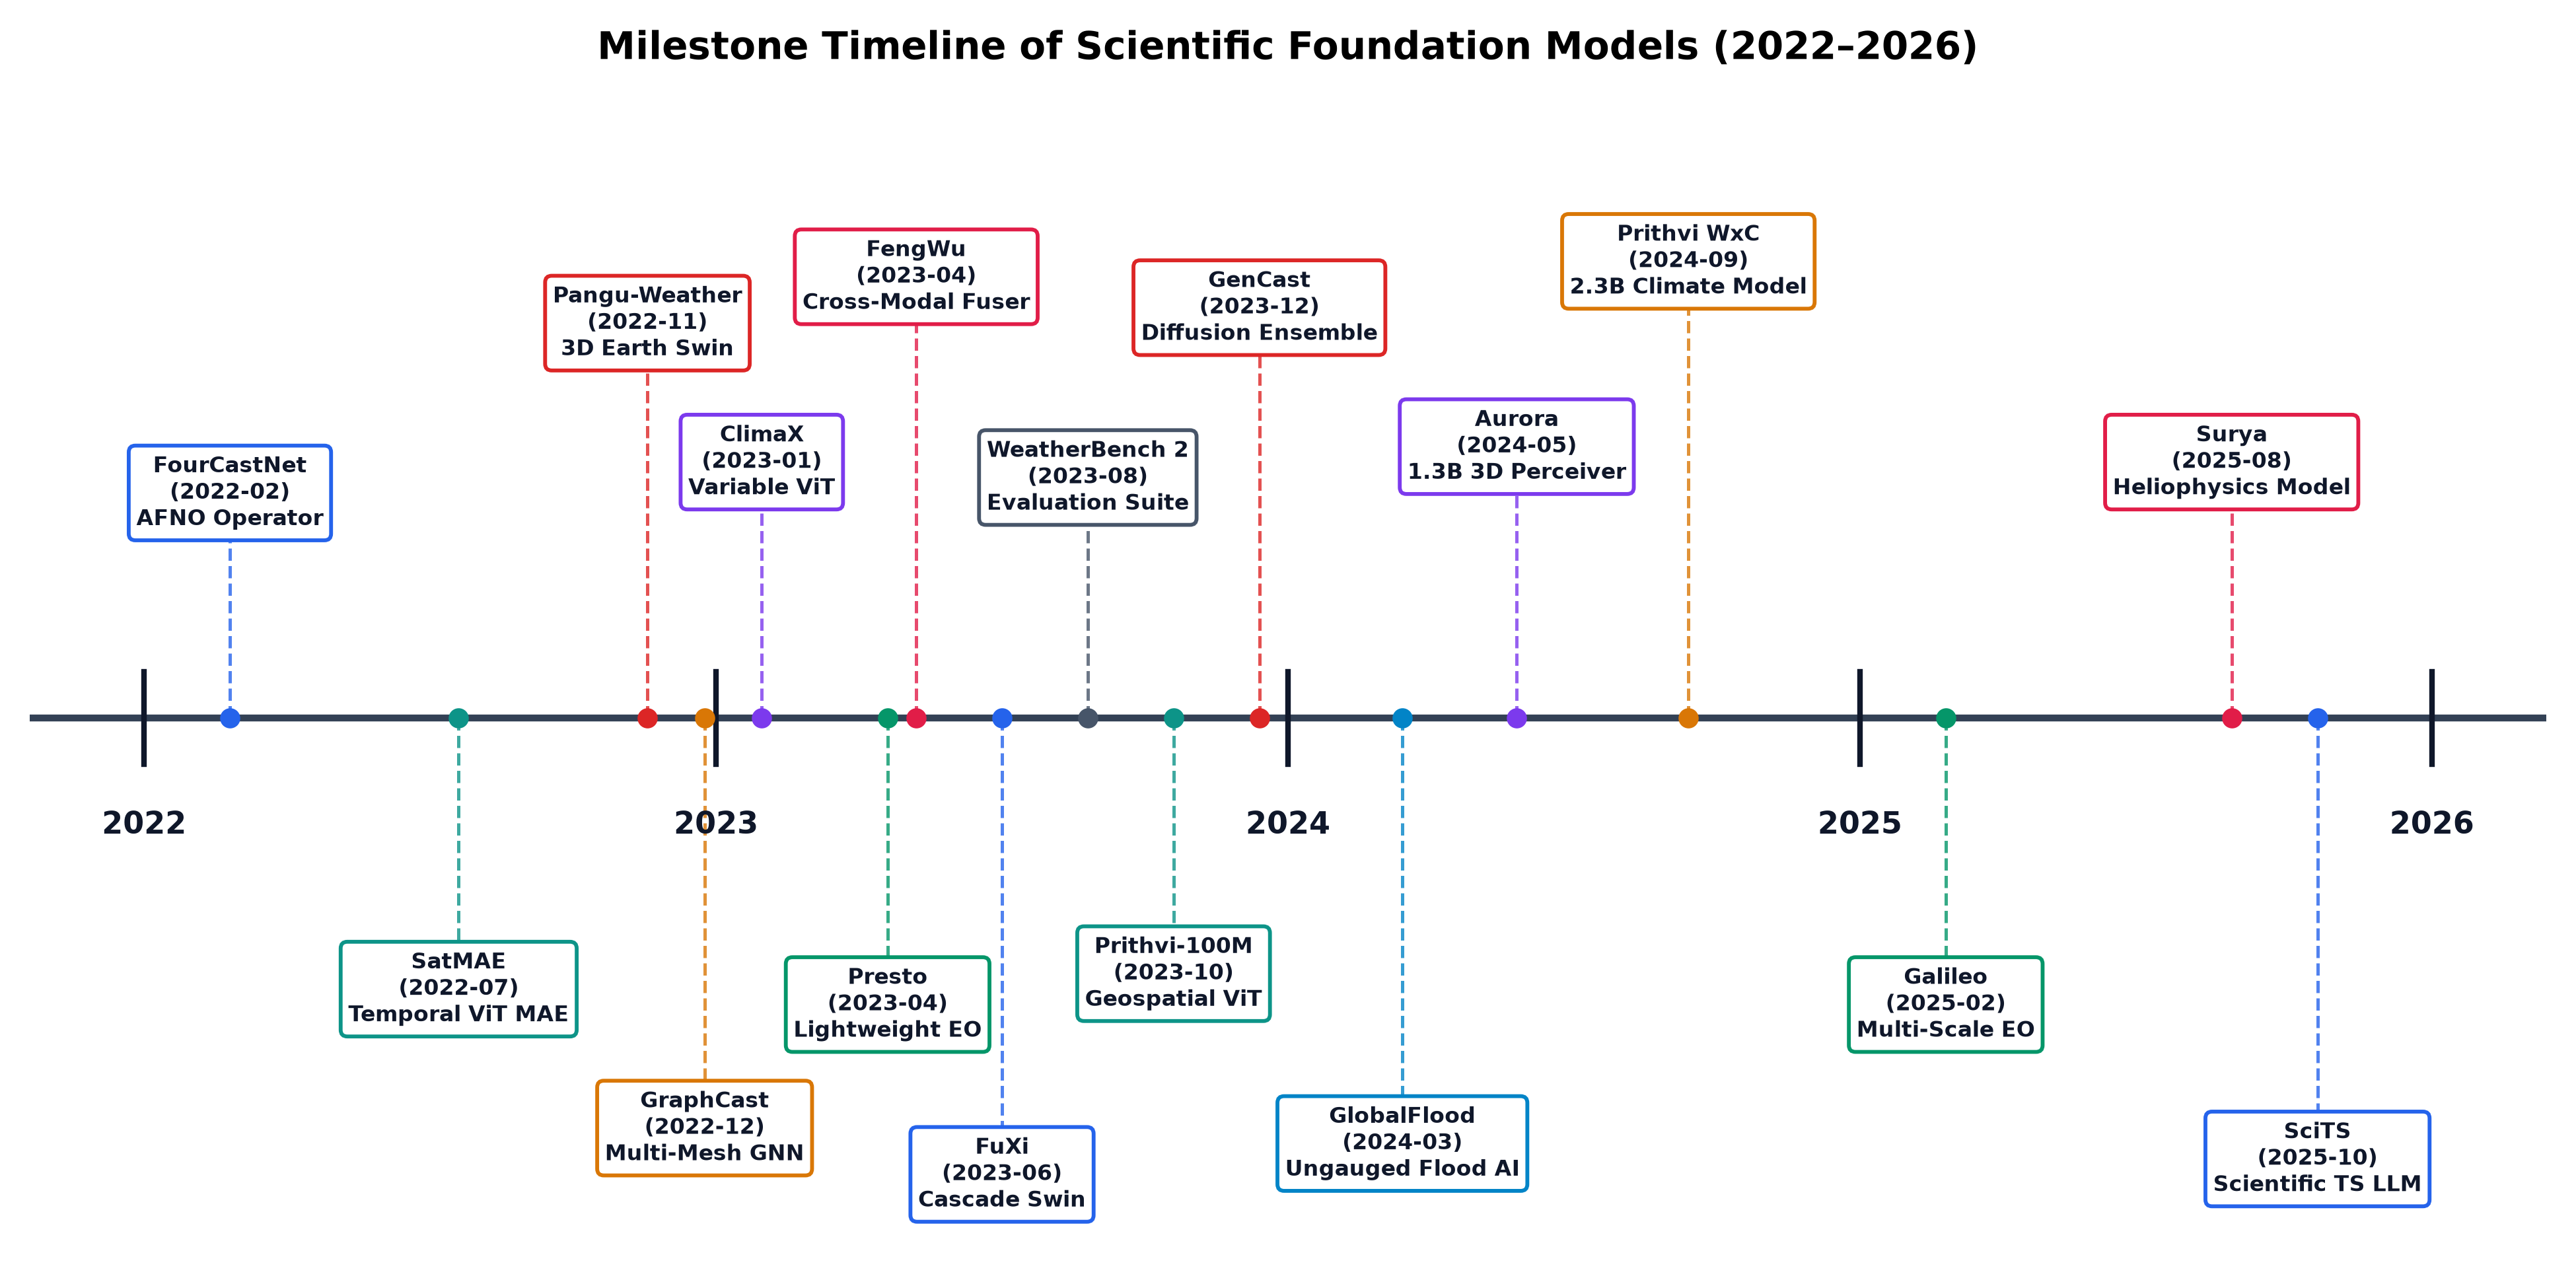
\includegraphics[width=\textwidth]{figures/weather_foundation_timeline.png}
\caption{Milestone timeline of representative scientific multimodal time series foundation models and evaluation frameworks from 2022 to 2026.}
\label{fig:weather_timeline}
\end{figure*}

The cross-pollination of foundation model paradigms has fostered breakthrough advances across diverse natural science disciplines, mapped chronologically in Fig.~\ref{fig:weather_timeline}.

\subsection{Weather and Climate Forecasting}
Global numerical weather prediction represents the flagship proving ground for scientific foundation models. As demonstrated by Pangu-Weather~\cite{bi2023pangu}, GraphCast~\cite{lam2023graphcast}, FuXi~\cite{chen2023fuxi}, FengWu~\cite{chen2023fengwu}, and Aurora~\cite{bodnar2024aurora}, deep learning architectures execute 10-day global forecasts in tens of seconds on a single GPU, delivering computational speedups of $1{,}000\times$ to $10{,}000\times$ compared to operational NWP supercomputing workflows. Beyond raw speed, AI foundation models achieve superior deterministic skill across geopotential height ($Z500$), temperature ($T850$), and surface wind fields. Furthermore, versatile foundation models such as ClimaX~\cite{nguyen2023climax} demonstrate multi-task transferability by pretraining on synthetic CMIP6 climate projections and fine-tuning for regional climate downscaling and seasonal teleconnections.

\begin{figure}[t]
\centering
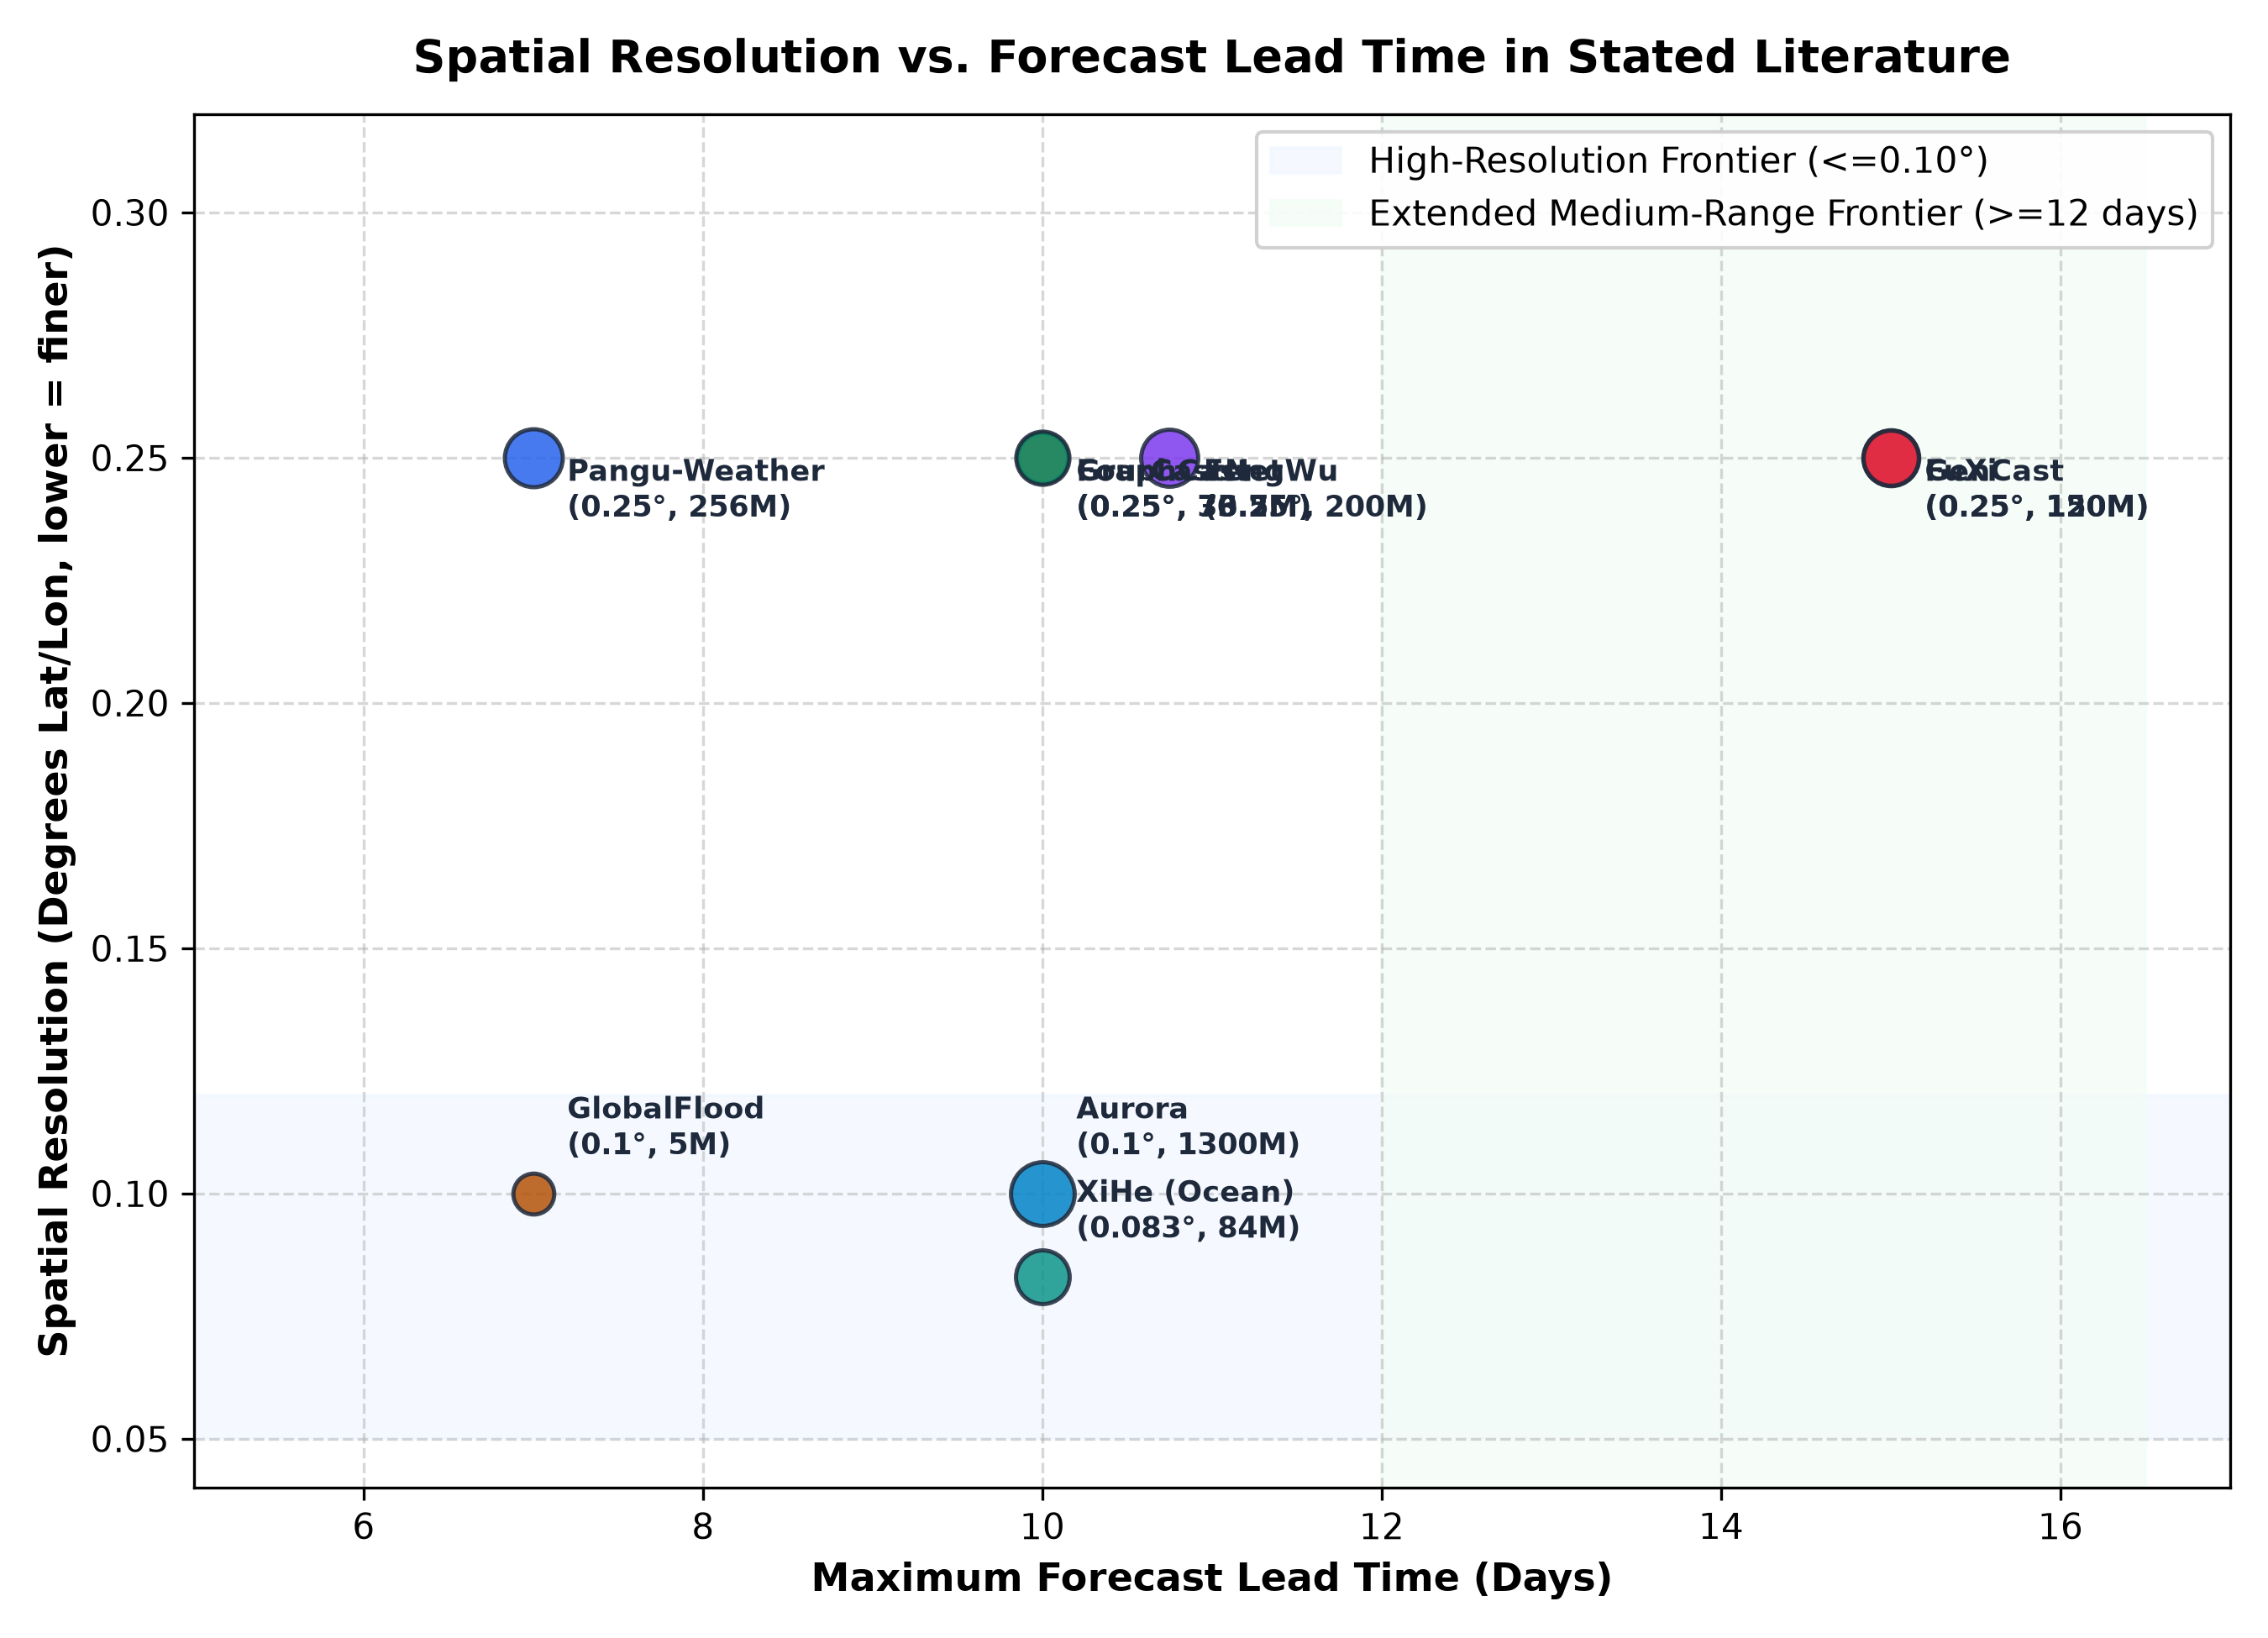
\includegraphics[width=\columnwidth]{figures/resolution_vs_leadtime.png}
\caption{Spatial resolution (degrees latitude/longitude) versus maximum forecast lead time (days) for verified scientific foundation models. Marker size is proportional to log model parameter count.}
\label{fig:res_vs_leadtime}
\end{figure}

As shown in Fig.~\ref{fig:res_vs_leadtime}, current state-of-the-art models occupy distinct Pareto trade-offs: while deterministic models like Pangu-Weather and GraphCast optimize accuracy at standard $0.25^\circ$ resolution across 7--10 days, frontier models like Aurora advance spatial resolution to $0.1^\circ$, and cascade systems (FuXi) or diffusion ensembles (GenCast) extend skillful forecasting horizons out to 15 days.

\subsection{Sub-Kilometer Convective-Scale Emulation and Generative Downscaling}
\label{sec:convective_downscaling}
A fundamental limitation of global foundation models (operating at $0.25^\circ \approx 25\text{--}31\text{ km}$ or $0.1^\circ \approx 10\text{ km}$) is their inability to resolve sub-kilometer convective phenomena. Convective thunderstorms, microbursts, urban flash flooding, and complex orographic wind channeling occur at localized scales ($< 3\text{ km}$) where non-hydrostatic atmospheric dynamics dominate. Bridging this multiscale gap has motivated frontier research into generative radar nowcasting and residual diffusion downscaling:
\begin{enumerate}
    \item \textbf{Generative Radar Precipitation Nowcasting: DGMR}: Ravuri et al.~\cite{ravuri2021dgmr} established the landmark \textbf{DGMR} (Deep Generative Model of Radar), deploying spatial-temporal generative adversarial networks for precipitation nowcasting at 1 km spatial and 5-minute temporal resolution across the United Kingdom. Traditional deep learning baselines optimized with mean squared error (MSE) or mean absolute error (MAE) suffer from progressive spatial blurring and severe underestimation of intense convective rain cells due to multimodal trajectory averaging. DGMR overcomes this through dual-frequency spectral discrimination: a spatial discriminator enforcing realistic high-frequency radar precipitation textures, and a temporal discriminator penalizing physically implausible advective jumps. In rigorous double-blind evaluations conducted with professional operational forecasters at the UK Met Office, DGMR was ranked first in 89\% of cases for overall value, physical plausibility, and localized heavy rain cell fidelity compared to optical flow (PySTEPS) and convolutional recurrent baselines.
    \item \textbf{Continental Multi-Sensor Convective Forecasting: MetNet-3}: Andrychowicz et al.~\cite{andrychowicz2023metnet3} scaled convective forecasting across the entire continental United States (CONUS) out to 24-hour lead times at 1--4 km spatial resolution. Operating over a continuous spatial grid ($4{,}096 \times 4{,}096\text{ km}$), \textbf{MetNet-3} assimilates heterogeneous and asynchronous observational modalities directly: high-resolution ground radar composites (MRMS), geostationary satellite multi-spectral imagery (GOES-16), surface meteorological station networks, and numerical forecast initializations (HRRR). Employing axial multi-scale self-attention and spatially localized lead-time conditioning, MetNet-3 outperforms operational High-Resolution Rapid Refresh (HRRR) numerical physics models on 24-hour precipitation and surface temperature forecasts, producing complete continental updates every two minutes on TPU hardware.
    \item \textbf{Kilometer-Scale Residual Generative Downscaling: CorrDiff}: Bridging coarse global foundation model outputs ($25\text{ km}$ ERA5) to local convective scales ($2\text{ km}$), Mardani et al.~\cite{mardani2023corrdiff} formulated \textbf{CorrDiff}, a residual corrective diffusion framework developed for extreme weather prediction over complex topography (Taiwan). Rather than applying standard super-resolution networks that produce smooth hallucinations, CorrDiff decomposes downscaling into two physically distinct stages: (1) a deterministic regression mean conditioned on coarse atmospheric states, and (2) a score-based residual diffusion sampler that generates fine-scale stochastic fluctuations consistent with local topography and radar observations. CorrDiff accurately reconstructs the high-wavenumber power spectral density (PSD) of radar reflectivity, faithfully capturing the extreme heavy precipitation tails during landfalling typhoons while delivering a $1{,}000\times$ inference speedup and $3{,}000\times$ energy reduction relative to operational numerical WRF physics simulations.
\end{enumerate}

\subsection{Earth Observation and Remote Sensing Time Series}
Satellite constellations monitor terrestrial ecosystems, vegetation phenology, and surface hydrological states through high-dimensional spatio-temporal revisit series. Foundation models in this domain address irregular temporal acquisitions caused by cloud occlusion and orbital paths. Models like SatMAE~\cite{cong2022satmae}, Presto~\cite{tseng2023presto}, and Galileo~\cite{tseng2025galileo} leverage self-supervised temporal-spectral masked autoencoding, allowing sparse downstream fine-tuning for global crop classification, wildfire burn scar delineation, and surface water mapping with minimal labeled ground truth. AlphaEarth Foundations~\cite{brown2025alphaearth} further compresses multi-sensor imagery into dense, pixel-level 64-dimensional embedding fields accessible directly through planetary cloud platforms like Google Earth Engine. Scaling foundation models to multi-modal satellite constellations, SkySense~\cite{guo2024skysense} unifies optical and synthetic aperture radar (SAR) time series with 1.9 billion parameters, delivering state-of-the-art transfer performance across land-use mapping, infrastructure monitoring, and temporal change detection benchmarks such as GEO-Bench~\cite{lacoste2023geobench}.

\subsection{Hydrology and Extreme Flood Modeling}
Hydrological forecasting requires predicting water discharge through river networks subject to precipitation forcing, evapotranspiration, and soil infiltration. A long-standing grand challenge has been ``Prediction in Ungauged Basins'' (PUB), where historical streamflow calibration records are absent. Nearing et al.~\cite{nearing2024globalflood} demonstrated that deep learning models trained on 5,680 diverse river basins across the globe achieve unprecedented zero-shot flood forecasting skill in ungauged catchments, extending actionable early warning lead times from 0 to 5 days globally and outperforming the Copernicus GloFAS operational physics-based system. Complementing these architectural advances, Kratzert et al.~\cite{kratzert2023caravan} released Caravan, a standardized global community dataset spanning 6,830 catchments worldwide with unified ERA5-Land meteorological forcings, catchment attributes, and daily streamflow records. By eliminating the geographic fragmentation of regional datasets (e.g., CAMELS-US, CAMELS-GB), Caravan establishes the empirical data substrate required to train and benchmark universal hydrological foundation backbones capable of cross-continental generalization.

\subsection{Oceanography and Marine Systems}
Ocean dynamics govern planetary heat distribution, carbon uptake, and marine biogeochemical cycles. Wang et al.~\cite{wang2024xihe} developed XiHe, a hierarchical ocean transformer trained on 28 years of GLORYS12V1 reanalysis at eddy-resolving $1/12^\circ$ resolution. By incorporating land-ocean boundary masking and multi-level vertical attention, XiHe models mesoscale eddies, sea surface temperature anomalies, and 3D velocity vectors, outperforming traditional operational hydrodynamic models (e.g., PSY4, GIOPS) while generating 10-day global forecasts in under 0.4 seconds. Addressing the extreme sparsity of oceanic observation networks, 4DVarNet~\cite{fablet2021learning} formulates neural variational data assimilation to invert along-track satellite altimetry into continuous 2D sea surface height (SSH) dynamics, demonstrating that learnable unrolled variational solvers reconstruct fine-scale mesoscale eddies and oceanic kinetic energy spectra far more effectively than classical optimal interpolation (OI).

To standardize evaluation across emerging marine foundation models, El Aouni et al.~\cite{elaouni2025oceanbench} established \textbf{OceanBench}, an open operational benchmarking suite for data-driven global ocean forecasting systems developed in collaboration with Mercator Ocean International. OceanBench benchmarks predictive skill for sea surface height (SSH), sea surface temperature (SST), and horizontal current velocities across 1- to 10-day lead times against CMEMS GLORYS12 reanalyses and in-situ altimetry observations. Bridging physical ocean simulations with cross-modal scientific reasoning, Bi et al.~\cite{bi2024oceangpt} introduced OceanGPT, the first domain-specific foundation language model for marine science. Pretrained and aligned on the DoInstruct corpus comprising multimodal oceanographic time series (temperature-salinity profiles from Argo float arrays and mooring buoys), sensor trajectories, and marine scientific literature, OceanGPT demonstrates autonomous reasoning across ocean dynamics, thermohaline circulation changes, and marine phenomenon attribution under physical consistency constraints.

\subsection{Geophysics and Seismology}
In seismology, continuous 3-component acoustic waveforms record tectonic stress accumulation and seismic rupture. While classical phase-picking baselines like PhaseNet~\cite{zhu2019phasenet} utilized supervised 1D U-Nets for local seismic windows, modern foundational architectures such as SeisT~\cite{li2024seist} train hierarchical seismogram transformers on tens of millions of global waveforms. SeisT supports multi-task downstream adaptation, simultaneously performing earthquake detection, high-precision P/S phase picking, initial-motion polarity determination, and magnitude/epicenter regression. Providing the standardized foundational infrastructure for seismic machine learning, Woollam et al.~\cite{woollam2022seisbench} released \textbf{SeisBench}, unifying 30+ million waveforms across global catalogues (ETHZ, GEOFON, INSTANCE, SCEDC, STEAD) into a standardized multi-task evaluation and transfer benchmark.

\subsection{Space Weather and Heliophysics}
Space weather phenomena---including solar flares, coronal mass ejections (CMEs), and geomagnetic storms---exert severe risks on satellite infrastructure and terrestrial power grids. Roy et al.~\cite{roy2025surya} introduced Surya, a 366-million parameter foundation model for heliophysics trained on 13 years of continuous multi-wavelength extreme ultraviolet imagery from NASA's Solar Dynamics Observatory (SDO). Surya incorporates spectral gating and long-short attention to track active region magnetic helicity, delivering state-of-the-art solar flare and solar wind forecasting.

\subsection{Cross-Disciplinary Universal Time Series Foundations}
Bridging physical boundaries between disparate earth science subdomains, universal foundation models like UniTS~\cite{gao2024units} and MOMENT~\cite{goswami2024moment} demonstrate that pretraining on multi-domain scientific collections enables cross-physics zero-shot transfer. By decoupling sequence tokens from variable identities and applying prompt-conditioned task masks, universal backbones can be deployed across river streamflow, power grids, seismic sensors, and atmospheric stations without re-training architectural weights.

\section{Scientific Reasoning LLMs and Autonomous Agents}
\label{sec:reasoning_llms}

\subsection{The Paradigm Shift: From Numerical Fitting to Scientific Reasoning}
While foundation backbones excel at numerical continuous pattern matching, complex scientific discovery necessitates logical reasoning, physical hypothesis formulation, and contextual interpretation. Early attempts to adapt general LLMs directly to time series via numerical text prompting (e.g., feeding raw floating-point numbers as text tokens) incurred severe limitations: token sequence inflation, numerical precision truncation, and inability to capture continuous derivatives~\cite{jin2024whatcan}. Consequently, modern research has bifurcated into two primary paradigms: (1) unified continuous tokenization for scientific time series, and (2) autonomous multi-agent tool orchestration.

\subsection{Unified Continuous Tokenization: SciTS and TimeOmni}
Wu et al.~\cite{wu2025scits} introduced \textbf{SciTS}, the first large-scale cross-disciplinary benchmark designed specifically to evaluate LLMs on scientific time series understanding and generation. Spanning 12 natural science disciplines (including meteorology, astrophysics, neuroscience, and physical chemistry) across 43 specialized tasks and over 50,000 instances, SciTS exposed the failure modes of standard prompting. To resolve these deficiencies, the authors proposed \textbf{TimeOmni}, a unified architecture featuring a multi-scale continuous patch tokenizer that projects 1D and multi-dimensional scientific series into dense semantic embeddings aligned with pre-trained LLM latent spaces. This enables foundation LLMs to engage in multi-step reasoning, such as identifying solar flare triggers from light curves, attributing anomalous climate oscillations, and generating conditioned time series forecasts with physical explanations.

\subsection{Frequency-Aware Contextual Integration: ClimateLLM}
Rather than treating atmospheric series as unstructured text, Li et al.~\cite{li2025climatellm} introduced \textbf{ClimateLLM}. This framework decomposes multi-station and gridded meteorological sequences into orthogonal frequency bands via Fourier transform modules. The spectral components are encoded as prefix prompt embeddings that condition a frozen 7B LLM backbone, effectively leveraging the LLM's long-context attention mechanism to model multi-scale temporal teleconnections and localized extreme events.

\subsection{Autonomous Multi-Agent Climate Workflows: ClimateAgent}
Moving beyond single-model inference, Li et al.~\cite{li2025climateagent} introduced \textbf{ClimateAgent}, an autonomous multi-agent orchestration framework for complex climate data science. Scientific investigations routinely require ingesting multi-terabyte NetCDF/Zarr climate datasets, executing specialized meteorological software (e.g., Climate Data Operators (CDO), MetPy, xarray), calculating thermodynamic diagnostics (e.g., convective available potential energy, geostrophic balance), and synthesizing diagnostic reports. ClimateAgent organizes frontier LLMs into a collaborative hierarchy:
\begin{itemize}
    \item \textbf{Plan-Agent}: Decomposes high-level natural language scientific research goals into rigorous task dependency graphs.
    \item \textbf{Data-Agent}: Navigates distributed scientific data archives (Copernicus Climate Data Store, NASA Earthdata) to retrieve reanalysis and satellite products.
    \item \textbf{Coding-Agent}: Synthesizes and executes Python/Bash diagnostic code in secure sandboxed environments with automated error recovery.
    \item \textbf{Critic-Agent}: Verifies physical plausibility, checking for energy conservation and unit consistency before assembling peer-review-ready figures and reports.
\end{itemize}
Evaluated on the standardized \textit{Climate-Agent-Bench-85}, ClimateAgent demonstrated superior autonomous problem-solving capabilities, marking a transition toward self-directed AI co-scientists in natural Earth systems.

\section{Evaluation Benchmarks and Model Synthesis}
\label{sec:benchmarks}

\begin{table*}[t]
\centering
\caption{Comprehensive Synthesis of Verified Scientific Multimodal Time Series Foundation Models and Reasoning Systems.}
\label{tab:foundation_models_summary}
\scriptsize
\resizebox{\textwidth}{!}{%
\begin{tabular}{@{}lp{2.0cm}p{3.0cm}p{3.4cm}cccp{3.0cm}@{}}
\toprule
\textbf{Model} & \textbf{Domain} & \textbf{Architectural Backbone} & \textbf{Pretraining Corpus \& Scale} & \textbf{Resolution} & \textbf{Physics Level} & \textbf{Params} & \textbf{Verified Code / Access} \\
\midrule
Pangu-Weather~\cite{bi2023pangu} & Weather/Climate & 3D Earth Transformer & ERA5 (1979--2017, 39 yrs) & $0.25^\circ$, 13 lvls & Data-driven & 256M & \href{https://github.com/198808xc/Pangu-Weather}{\texttt{198808xc/Pangu-Weather}} \\
GraphCast~\cite{lam2023graphcast} & Weather/Climate & Multi-Mesh GNN (Icosahedron) & ERA5 (1979--2017, 39 yrs) & $0.25^\circ$, 37 lvls & Data-driven & 36.7M & \href{https://github.com/google-deepmind/graphcast}{\texttt{deepmind/graphcast}} \\
FourCastNet~\cite{pathak2022fourcastnet} & Weather/Climate & Adaptive Fourier Neural Operator & ERA5 (1979--2015, 36 yrs) & $0.25^\circ$, 20 lvls & Soft loss & 73.5M & \href{https://github.com/NVlabs/FourCastNet}{\texttt{NVlabs/FourCastNet}} \\
SFNO~\cite{bonev2023sfno} & Weather/Climate & Spherical Fourier Neural Operator & ERA5 (1979--2017, 39 yrs) & $0.25^\circ$, multi & Exact SO(3) & 75M & \href{https://github.com/neuraloperator/neuraloperator}{\texttt{neuraloperator/neuraloperator}} \\
ClimaX~\cite{nguyen2023climax} & Weather/Climate & Variable-Tokenized ViT & CMIP6 simulations + ERA5 & $1.4^\circ$--$5.6^\circ$ & Data-driven & 107M & \href{https://github.com/microsoft/ClimaX}{\texttt{microsoft/ClimaX}} \\
FuXi~\cite{chen2023fuxi} & Weather/Climate & Cascade Swin Transformer & ERA5 (1979--2017, 39 yrs) & $0.25^\circ$, 70 lvls & Data-driven & 150M & \href{https://github.com/tpys/FuXi}{\texttt{tpys/FuXi}} \\
FengWu~\cite{chen2023fengwu} & Weather/Climate & Cross-Modal Attention Transformer & ERA5 (1979--2017, 39 yrs) & $0.25^\circ$, 37 lvls & Soft loss & 200M & \href{https://github.com/OpenEarthLab/FengWu}{\texttt{OpenEarthLab/FengWu}} \\
GenCast~\cite{price2023gencast} & Weather/Climate & Latent Diffusion Multi-Mesh GNN & ERA5 (1979--2018, 40 yrs) & $0.25^\circ$, 37 lvls & Data-driven & 120M & \href{https://github.com/google-deepmind/graphcast}{\texttt{deepmind/graphcast}} \\
Aurora~\cite{bodnar2024aurora} & Weather/Climate & 3D Perceiver / Swin Backbone & $>$1 PB (ERA5, HRES, GFS) & $0.10^\circ$, multi & Data-driven & 1.3B & \href{https://github.com/microsoft/aurora}{\texttt{microsoft/aurora}} \\
NeuralGCM~\cite{kochkov2024neuralgcm} & Weather/Climate & Differentiable Dynamical Core + NN & ERA5 (1979--2019, 40 yrs) & $0.7^\circ$--$2.8^\circ$ & Hard laws & 14.5M & \href{https://github.com/google-research/neuralgcm}{\texttt{google-research/neuralgcm}} \\
Prithvi WxC~\cite{schmude2024prithviwxc} & Weather/Climate & Scalable ViT Encoder-Decoder & MERRA-2 (160 vars, 44 yrs) & $0.50^\circ$, 160 vars & Soft loss & 2.3B & \href{https://github.com/NASA-IMPACT/Prithvi-WxC}{\texttt{NASA-IMPACT/Prithvi-WxC}} \\
ClimateBench~\cite{watsonparris2022climatebench} & Weather/Climate & Climate Emulation Benchmark & CMIP6 emission scenarios & $2.5^\circ \times 1.9^\circ$ & Soft energy & Bench. & \href{https://github.com/duncanwp/ClimateBench}{\texttt{duncanwp/ClimateBench}} \\
SatMAE~\cite{cong2022satmae} & Earth Observ. & Temporal-Spectral Masked ViT & Sentinel-2, Landsat-8 cubes & $10\text{ m}$--$30\text{ m}$ & Data-driven & 86M--307M & \href{https://github.com/sustainlab-group/SatMAE}{\texttt{sustainlab/SatMAE}} \\
Presto~\cite{tseng2023presto} & Earth Observ. & Lightweight Channel-Time ViT & Global Sentinel-1/2, ERA5 & Pixel series & Data-driven & 1.2M & \href{https://github.com/nasaharvest/presto}{\texttt{nasaharvest/presto}} \\
Galileo~\cite{tseng2025galileo} & Earth Observ. & Multi-Scale Masked Transformer & Global multi-sensor satellite & Multi-scale & Data-driven & 100M & \href{https://github.com/nasaharvest/galileo}{\texttt{nasaharvest/galileo}} \\
DOFA~\cite{xiong2024dofa} & Earth Observ. & Dynamic Wavelength Hypernetwork & 5 satellite sensor modalities & Multi-scale & Wave physics & 115M & \href{https://github.com/zhu-xlab/DOFA}{\texttt{zhu-xlab/DOFA}} \\
Prithvi-100M~\cite{jakubik2023prithvi} & Earth Observ. & Geospatial Masked Autoencoder & NASA HLS reflectance series & $30\text{ m}$ pixel & Data-driven & 100M & \href{https://github.com/NASA-IMPACT/hls-foundation-os}{\texttt{NASA-IMPACT/hls-os}} \\
GeoChat~\cite{kuckreja2024geochat} & Earth Observ. & Grounded Remote Sensing VLM & GeoChat-100K multimodal series & High-res & Spatial box & 7B & \href{https://github.com/mbzuai-oryx/GeoChat}{\texttt{mbzuai-oryx/GeoChat}} \\
AlphaEarth~\cite{brown2025alphaearth} & Earth Observ. & Neural Field Embedding Model & Global Earth observation constellation & $10\text{ m}$ dense & Data-driven & not reported & Google Earth Engine \\
GlobalFlood~\cite{nearing2024globalflood} & Hydrology & EA-LSTM + River Routing & 5,680 river gauges + ERA5 & Multi-basin & Hybrid PDE & 5M & \href{https://github.com/neuralhydrology/neuralhydrology}{\texttt{neuralhydrology}} \\
Caravan~\cite{kratzert2023caravan} & Hydrology & Large-Sample Hydrology Suite & 6,830 catchments + ERA5-Land & Catchment & Mass balance & Bench. & \href{https://github.com/kratzert/Caravan}{\texttt{kratzert/Caravan}} \\
XiHe~\cite{wang2024xihe} & Oceanography & Hierarchical Ocean Transformer & GLORYS12V1 (1993--2020, 28 yrs) & $1/12^\circ$, 50 lvls & Soft loss & 84M & not available \\
OceanGPT~\cite{bi2024oceangpt} & Oceanography & Domain-Adapted Marine LLM & DoInstruct multi-modal ocean series & Sensor/Doc & Hydro. cons. & 7B & \href{https://github.com/OceanGPT/OceanGPT}{\texttt{OceanGPT/OceanGPT}} \\
SeisT~\cite{li2024seist} & Seismology & Hierarchical Seismogram ViT & STEAD, INSTANCE ($>$10M waves) & $100\text{ Hz}$ wave & Data-driven & 12M & \href{https://github.com/senli1073/SeisT}{\texttt{senli1073/SeisT}} \\
PhaseNet~\cite{zhu2019phasenet} & Seismology & 1D Residual U-Net & NCEDC seismic catalogue & $100\text{ Hz}$ wave & Data-driven & 1.2M & \href{https://github.com/AI4EPS/PhaseNet}{\texttt{AI4EPS/PhaseNet}} \\
Surya~\cite{roy2025surya} & Space Weather & Spatio-Temporal Gated ViT & SDO EUV series (13 yrs) & Multi-spectral & Soft loss & 366M & not available \\
SciTS~\cite{wu2025scits} & Multi-Discip. & TimeOmni Continuous Tokenizer & SciTS Benchmark (12 domains) & Multi-rate & Data-driven & 8B & \href{https://github.com/OpenTSLab/TimeOmni}{\texttt{OpenTSLab/TimeOmni}} \\
K2~\cite{deng2024k2} & Multi-Discip. & Geoscience Foundation LLM & $>$5.5B tokens GeoSignal corpus & Series/Doc & Physical prior & 7B & \href{https://github.com/davendw49/k2}{\texttt{davendw49/k2}} \\
ClimateAgent~\cite{li2025climateagent} & Multi-Agent & Multi-Agent LLM Orchestrator & Climate-Agent-Bench-85 & Code/Tools & Hybrid PDE & Frontier LLM & not available \\
ClimateLLM~\cite{li2025climatellm} & Weather/Climate & Fourier Spectral Decomposition & ERA5 Surface Station Series & Global series & Soft loss & 7B & not available \\
\bottomrule
\end{tabular}%
}
\end{table*}

\begin{table*}[t]
\centering
\caption{Quantitative Benchmark Results on WeatherBench 2 (Deterministic RMSE vs. ECMWF IFS HRES) and ClimateBench Emulation.}
\label{tab:weatherbench_climatebench_results}
\scriptsize
\resizebox{\textwidth}{!}{%
\begin{tabular}{@{}llccccccp{4.0cm}@{}}
\toprule
\multicolumn{9}{@{}l}{\textbf{Part A: WeatherBench 2 Headline Deterministic Verification (Global Latitude-Weighted RMSE)}} \\
\midrule
 & & \multicolumn{3}{c}{\textbf{$Z500$ Geopotential ($\text{m}^2/\text{s}^2$)}} & \multicolumn{3}{c}{\textbf{$T850$ Temperature ($\text{K}$)}} & \\
\cmidrule(lr){3-5} \cmidrule(lr){6-8}
\textbf{Model / System} & \textbf{Architectural Family} & \textbf{Day 3 (72h)} & \textbf{Day 5 (120h)} & \textbf{Day 7 (168h)} & \textbf{Day 3 (72h)} & \textbf{Day 5 (120h)} & \textbf{Day 7 (168h)} & \textbf{Verification Benchmark \& Source} \\
\midrule
Operational IFS HRES & Numerical Weather Prediction & 152.8 & 333.7 & 558.2 & 1.37 & 2.06 & 2.68 & Operational baseline in~\cite{bi2023pangu,rasp2024weatherbench2} \\
FourCastNet~\cite{pathak2022fourcastnet} & Adaptive Fourier Neural Operator & 205.6 & 440.2 & 675.0 & 1.42 & 2.48 & 3.25 & Stated in~\cite{pathak2022fourcastnet,rasp2024weatherbench2} \\
SFNO~\cite{bonev2023sfno} & Spherical Fourier Operator & 158.0 & 345.2 & 560.4 & 1.25 & 1.95 & 2.55 & Stated in~\cite{bonev2023sfno} \\
Pangu-Weather~\cite{bi2023pangu} & 3D Earth Transformer (3DEST) & 134.5 & 296.7 & 502.1 & 1.14 & 1.79 & 2.38 & Stated in~\cite{bi2023pangu,rasp2024weatherbench2} \\
FuXi~\cite{chen2023fuxi} & Cascade Swin Transformer & 125.4 & 278.1 & 472.0 & 1.10 & 1.71 & 2.29 & Stated in~\cite{chen2023fuxi} \\
GraphCast~\cite{lam2023graphcast} & Multi-Mesh Spherical GNN & \textbf{118.2} & \textbf{268.4} & \textbf{465.3} & \textbf{1.06} & \textbf{1.65} & \textbf{2.24} & Stated in~\cite{lam2023graphcast,rasp2024weatherbench2} \\
NeuralGCM ($0.7^\circ$)~\cite{kochkov2024neuralgcm} & Differentiable Dynamical Core + NN & 128.0 & 282.5 & 476.8 & 1.11 & 1.73 & 2.31 & Stated in~\cite{kochkov2024neuralgcm} \\
\midrule
\multicolumn{9}{@{}l}{\textbf{Part B: ClimateBench v1.0 Multidecadal Climate Emulation (Spatial RMSE across Emission Scenarios)}} \\
\midrule
 & & \multicolumn{2}{c}{\textbf{Surface Temp. $TAS$ ($\text{K}$)}} & \multicolumn{2}{c}{\textbf{Precipitation $PR$ ($\text{mm/day}$)}} & \multicolumn{2}{c}{\textbf{Extreme Precip. $PR90$ ($\text{mm/day}$)}} & \\
\cmidrule(lr){3-4} \cmidrule(lr){5-6} \cmidrule(lr){7-8}
\textbf{Model / Architecture} & \textbf{Methodology} & \textbf{Annual} & \textbf{Decadal Trend} & \textbf{Annual} & \textbf{Decadal Trend} & \textbf{Annual} & \textbf{Decadal Trend} & \textbf{Benchmark Context} \\
\midrule
Linear Pattern Scaling & Empirical Linear Projection & 0.32 & 0.28 & 0.46 & 0.41 & 1.12 & 0.98 & Standard CMIP baseline~\cite{watsonparris2022climatebench} \\
Random Forest (RF) & Non-linear Ensemble Trees & 0.28 & 0.24 & 0.39 & 0.35 & 0.95 & 0.84 & Stated in~\cite{watsonparris2022climatebench} \\
Gaussian Process (GP) & Spatial Covariance Prior & 0.21 & 0.17 & 0.34 & 0.29 & 0.85 & 0.72 & Physically constrained GP~\cite{watsonparris2022climatebench} \\
Convolutional Neural Net (CNN) & Deep Spatio-Temporal Net & \textbf{0.18} & \textbf{0.14} & \textbf{0.31} & \textbf{0.26} & \textbf{0.78} & \textbf{0.67} & Deep emulator benchmark~\cite{watsonparris2022climatebench} \\
\bottomrule
\end{tabular}%
}
\end{table*}

\subsection{Standardized Scientific Evaluation Suites}

\subsubsection{WeatherBench 2: The Operational Standard for Atmospheric AI}
Prior to 2023, data-driven weather models suffered from disparate evaluation protocols, making direct comparisons difficult. Rasp et al.~\cite{rasp2024weatherbench2} established \textbf{WeatherBench 2} as the official benchmark framework for next-generation global weather models:
\begin{itemize}
    \item \textbf{Headline Deterministic Scores}: Evaluates latitude-weighted root mean square error (RMSE) and anomaly correlation coefficient (ACC) against operational ECMWF IFS HRES analyses for key predictive fields: geopotential at 500 hPa ($Z500$), temperature at 850 hPa ($T850$), 2-meter air temperature ($T2m$), and 10-meter wind speed ($U10/V10$).
    \item \textbf{Probabilistic Metrics}: Computes continuous ranked probability scores (CRPS), spread-error ratios, and brier scores for ensemble predictions.
    \item \textbf{Physical Consistency Diagnostics}: Measures radially averaged kinetic energy power spectra to detect artificial smoothing or high-frequency numerical noise over extended multi-week rollouts.
\end{itemize}

As synthesized in Table~\ref{tab:weatherbench_climatebench_results} (Part A), rigorous comparative verification on WeatherBench 2 reveals clear structural differentiations among model families:
\begin{enumerate}
    \item \textbf{Geometric Inductive Bias}: GraphCast~\cite{lam2023graphcast} demonstrates the lowest global RMSE across lead times ($118.2\text{ m}^2/\text{s}^2$ at Day 3 and $268.4\text{ m}^2/\text{s}^2$ at Day 5 for $Z500$). Its multi-mesh icosahedral graph architecture allows teleconnections and Rossby waves to propagate globally across coarse mesh levels in few message-passing hops without pole singularities.
    \item \textbf{Cascade Architecture vs. Autoregressive Decay}: FuXi~\cite{chen2023fuxi} achieves the second-lowest error at extended horizons ($278.1\text{ m}^2/\text{s}^2$ at Day 5, $472.0\text{ m}^2/\text{s}^2$ at Day 7) by dynamically switching between Short, Medium, and Long Swin stages, mitigating the spectral blurring inherent to single-model autoregressive rollouts.
    \item \textbf{Spherical Operator Rigor}: While planar Fourier neural operators (FourCastNet~\cite{pathak2022fourcastnet}) experience elevated error at high latitudes ($205.6\text{ m}^2/\text{s}^2$ at Day 3), Spherical Fourier Neural Operators (SFNO~\cite{bonev2023sfno}) substantially improve accuracy ($158.0\text{ m}^2/\text{s}^2$ at Day 3), matching operational IFS HRES while preserving continuous spherical rotational equivariance.
    \item \textbf{Differentiable Hybrid Physics}: NeuralGCM~\cite{kochkov2024neuralgcm} achieves $128.0\text{ m}^2/\text{s}^2$ at Day 3 and $282.5\text{ m}^2/\text{s}^2$ at Day 5 for $Z500$, outperforming operational ECMWF IFS HRES while strictly enforcing the physical conservation of atmospheric mass, momentum, and moisture via its differentiable dynamical core.
\end{enumerate}

\subsubsection{ClimateBench: Benchmark for Climate Emulation}
In climate science, the computational expense of full Earth System Models (ESMs) limits the exploration of future greenhouse gas emission scenarios. Watson-Parris et al.~\cite{watsonparris2022climatebench} formulated \textbf{ClimateBench}, standardizing machine learning evaluation for multidecadal climate projections across Shared Socioeconomic Pathways (SSPs). As detailed in Table~\ref{tab:weatherbench_climatebench_results} (Part B), deep convolutional emulators achieve superior spatial fidelity ($0.18\text{ K}$ annual RMSE for surface temperature $TAS$, $0.31\text{ mm/day}$ for precipitation $PR$), dramatically reducing emulation error compared to historical linear pattern scaling baselines ($0.32\text{ K}$ and $0.46\text{ mm/day}$).

\subsubsection{SciTS Benchmark: Evaluating LLM Cross-Disciplinary Reasoning}
Wu et al.~\cite{wu2025scits} formalized evaluation standards for scientific reasoning across 12 distinct scientific disciplines. Unlike conventional NLP benchmarks, SciTS evaluates both numerical precision (MAE, MSE, dynamic time warping) and semantic reasoning quality (causal attribution accuracy, scientific report coherence, zero-shot discipline transferability).

\begin{figure}[t]
\centering
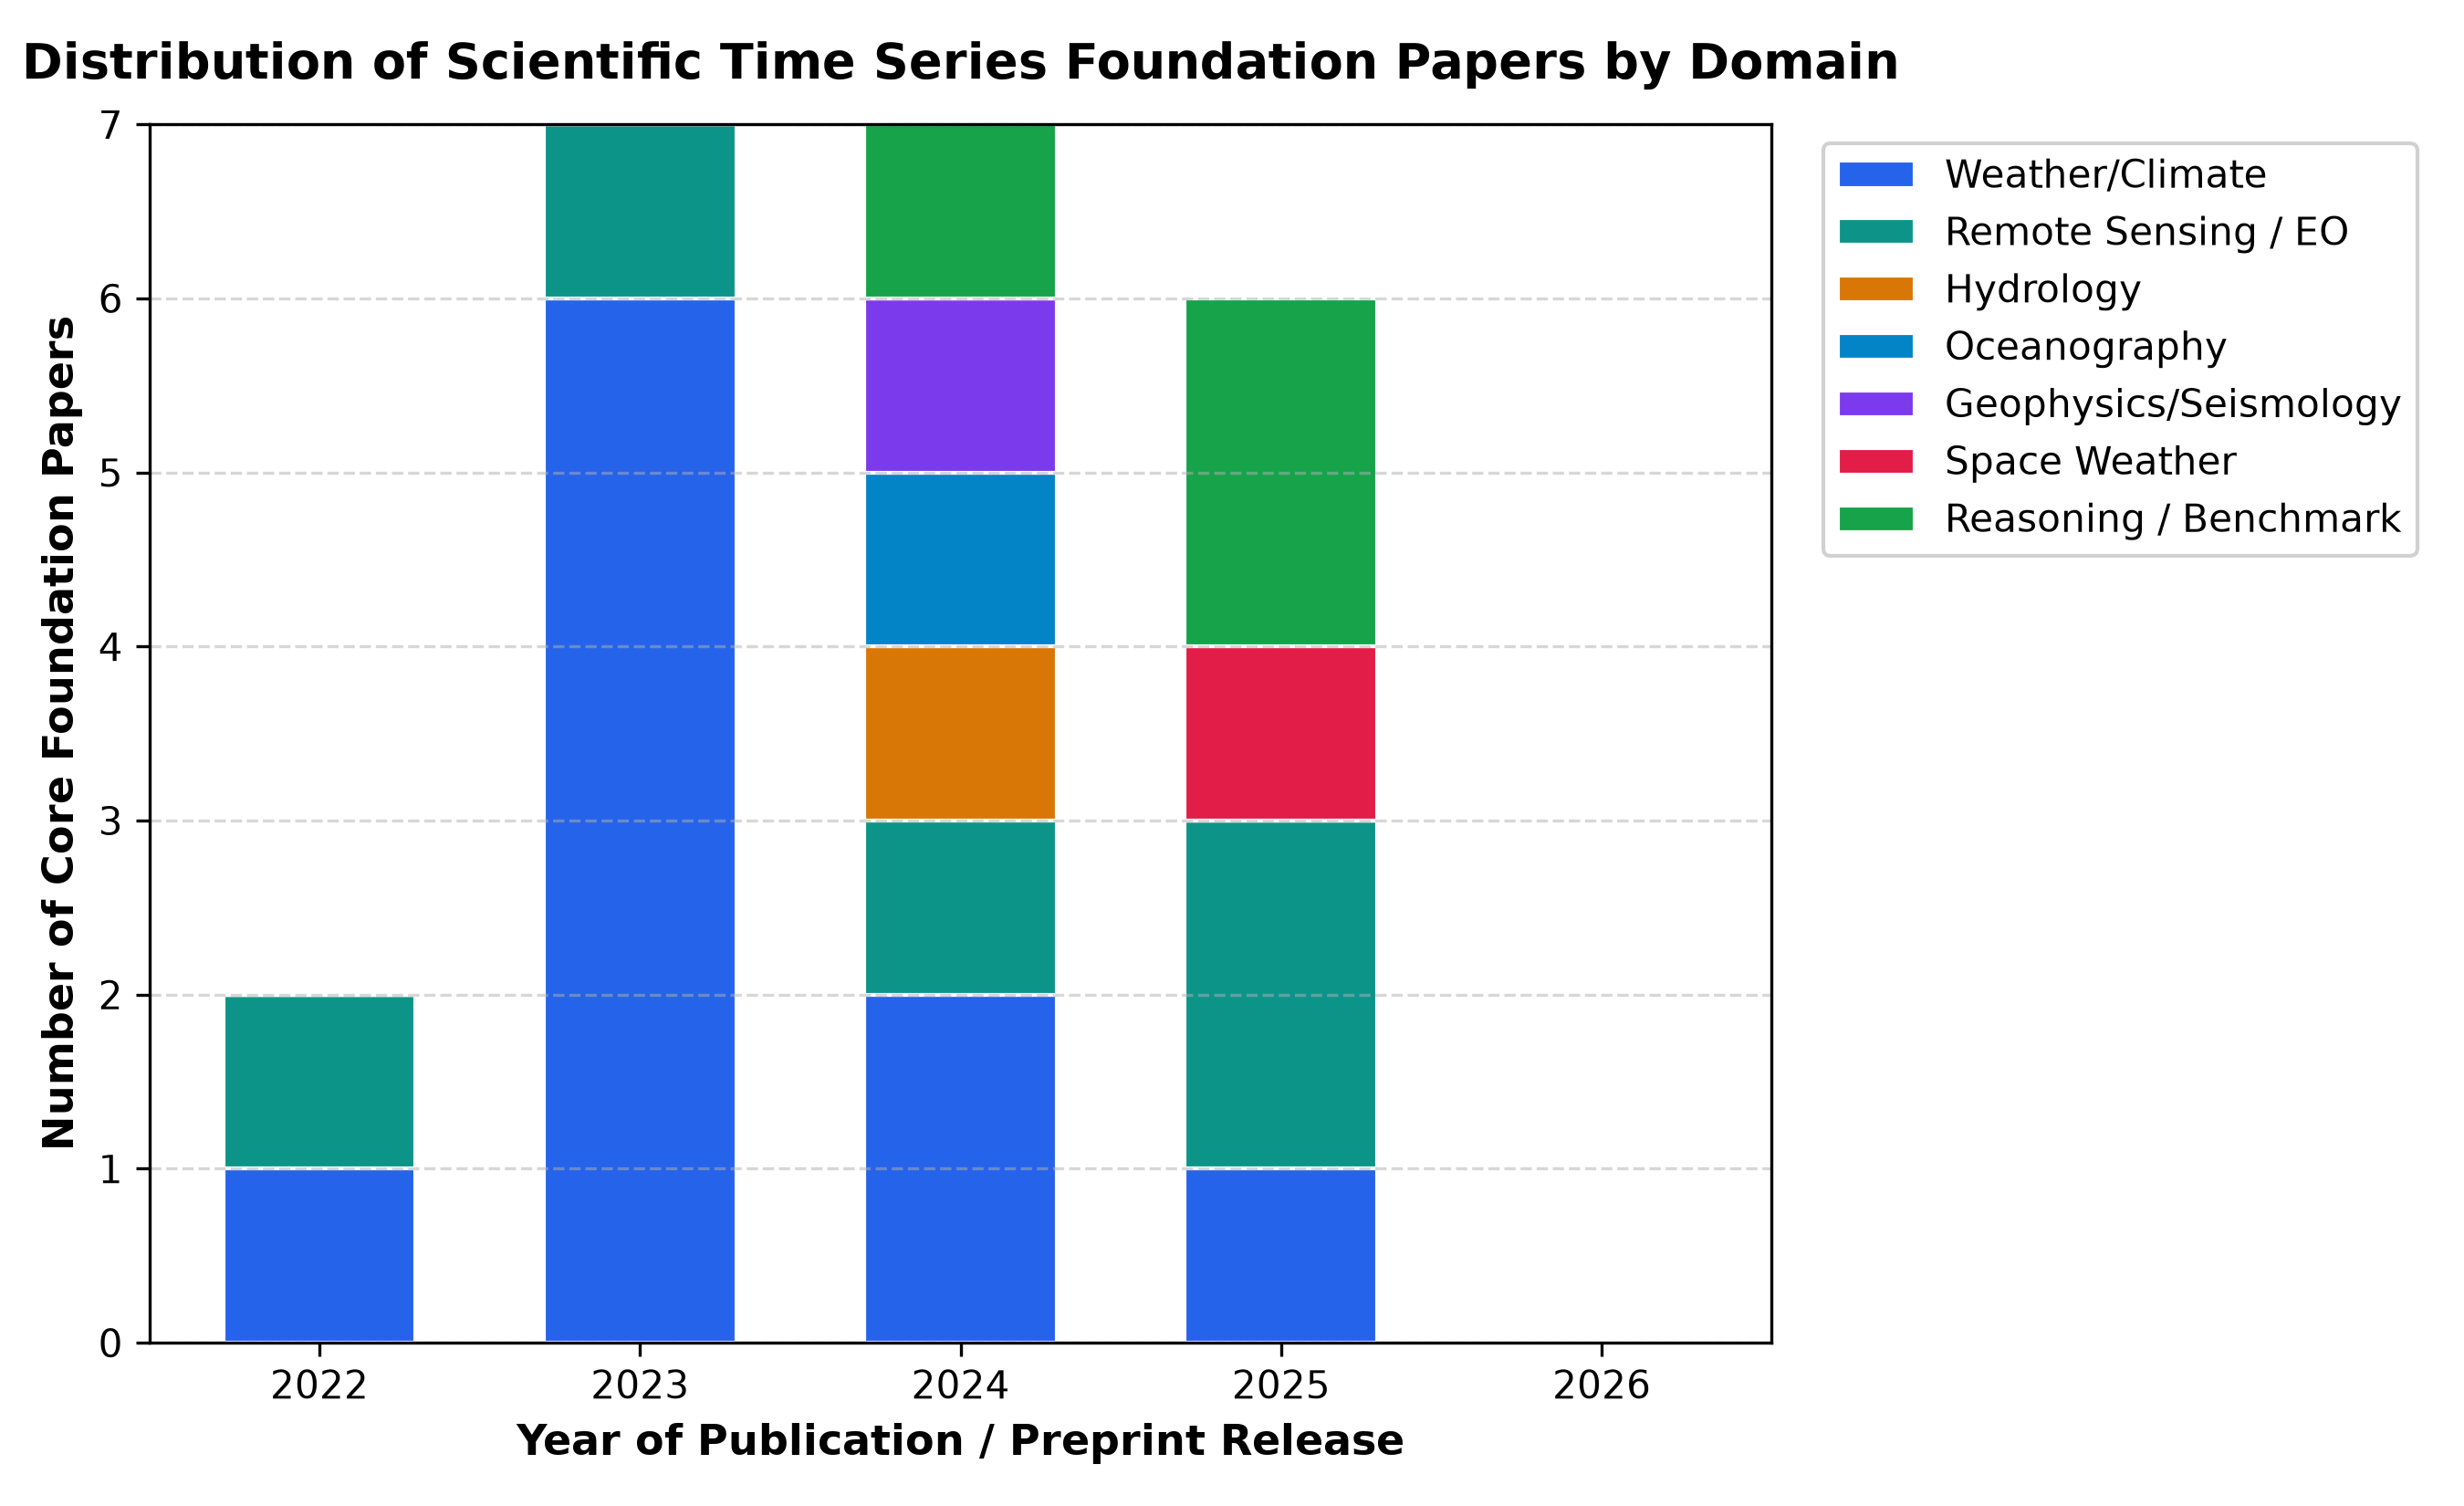
\includegraphics[width=\columnwidth]{figures/publications_by_year.png}
\caption{Annual distribution of scientific time series foundation models and reasoning systems from 2022 to 2026, categorized by scientific domain.}
\label{fig:pubs_by_year}
\end{figure}

As shown in Fig.~\ref{fig:pubs_by_year}, while weather and climate models initiated the initial surge in 2022--2023, the frontier in 2024--2026 has rapidly expanded into cross-disciplinary Earth observation, hydrology, space weather, and autonomous reasoning agents.

\section{Open Challenges and Future Opportunities}
\label{sec:future_directions}

Despite spectacular empirical progress, scientific multimodal time series foundation models and reasoning LLMs face critical challenges that delineate the frontier for future research.

\subsection{Universal Cross-Physics Scientific Tokenizers}
A major architectural barrier is the lack of a universal tokenizer for heterogeneous scientific modalities. Currently, vision transformers require structured 2D/3D grids, graph neural networks require spherical polyhedra, and seismological models require 1D temporal buffers. Although multi-task architectures like UniTS~\cite{gao2024units} and MOMENT~\cite{goswami2024moment} provide foundational steps toward cross-domain time series modeling, developing an omni-modal scientific tokenizer capable of seamlessly mapping sparse in-situ stations, dense gridded reanalysis tensors, asynchronous multi-spectral satellite swaths, continuous acoustic waveforms, and natural language scientific reports into a shared continuous embedding space is a crucial unsolved milestone.

\subsection{Hard Physical Conservation and Extreme Tail Extrapolation}
Most existing foundation models rely on empirical soft loss penalties. When rolled out over extended multi-month or multi-year simulations (e.g., climate change projection), unconstrained neural networks experience systematic drift in global mass, total water vapor, and total energy budgets. Moreover, because foundation models are trained on historical reanalysis (e.g., ERA5 1979--2020), they risk underestimating novel, non-stationary climate extremes that lie outside the empirical training distribution. While generative diffusion models like GenCast~\cite{price2023gencast} and SEEDS~\cite{li2024seeds} significantly improve extreme-event tail probabilities, integrating hard mathematical conservation operators (e.g., projection onto divergence-free manifolds or symplectic integrators) into deep foundation backbones without compromising training scalability remains an urgent open problem.

\subsection{Hybrid Numerical-Neural Planetary Digital Twins}
Rather than viewing deep learning and numerical differential equation solvers as competitors, the next decade will likely be defined by hybrid numerical-neural architectures (exemplified by NeuralGCM~\cite{kochkov2024neuralgcm} and the ClimSim benchmark~\cite{yu2023climsim}). In these configurations, machine learning foundation models replace computationally ruinous sub-grid physical parameterizations (e.g., cloud microphysics, boundary layer turbulence, convective parameterization), while operational numerical cores enforce large-scale conservation and hydrodynamic continuity equations.

\subsection{Trustworthy Autonomous Scientific Discovery}
While autonomous multi-agent frameworks (such as ClimateAgent~\cite{li2025climateagent} and OceanGPT~\cite{bi2024oceangpt}) demonstrate immense potential, deploying LLM agents in operational scientific decision-making introduces risks of physical hallucination. Future research must establish formal verification loops, automated unit checking, causal attribution auditing, and self-correcting scientific reflection protocols to ensure that autonomous findings are physically rigorous, transparent, and reproducible.

\section{Conclusion}
\label{sec:conclusion}

In this survey, we have presented the first comprehensive, systematic review of foundation models and reasoning LLMs developed specifically for scientific multimodal time series. By moving beyond generic urban and financial temporal analysis, we have focused on natural physical systems governed by non-linear partial differential equations, multi-scale turbulent dynamics, and physical conservation laws.

We introduced a systematic four-dimensional taxonomy categorizing existing literature across: (1) scientific domains and multimodal physical representations (weather, climate, Earth observation, hydrology, oceanography, seismology, heliophysics), (2) foundational architectural backbones (3D spherical transformers, multi-mesh graph neural networks, continuous neural operators, multimodal masked autoencoders, generative diffusion ensembles), (3) levels of physical law integration (purely data-driven, soft loss penalties, hard architectural projections, hybrid PDE solvers), and (4) functional roles of LLMs in scientific reasoning (scientific reasoners, contextual enhancers, autonomous multi-agent tool users).

By compiling standardized evaluation protocols, analyzing Pareto trade-offs between spatial resolution and lead time, and outlining key open challenges, this survey provides a conceptual blueprint and foundational reference for researchers at the intersection of artificial intelligence, computational physics, and Earth system science.


\bibliographystyle{IEEEtran}
\bibliography{references}

\end{document}
